\documentclass[10pt,a4paper,twocolumn]{article}

\usepackage[margin=0.72in]{geometry}
\usepackage{graphicx}
\usepackage{booktabs}
\usepackage{longtable}
\usepackage{array}
\usepackage{tabularx}
\usepackage{float}
\usepackage{amsmath}
\usepackage{enumitem}
\usepackage{caption}
\usepackage{hyperref}
\usepackage{setspace}
\usepackage{subfiles}

\hypersetup{
    colorlinks=true,
    linkcolor=blue,
    urlcolor=blue,
    citecolor=blue
}

\captionsetup{font=small, labelfont=bf}
\setlength{\parindent}{0pt}
\setlength{\parskip}{0.35em}
\setlength{\columnsep}{0.24in}
\setlist[itemize]{topsep=0.3em, itemsep=0.3em}

\newcolumntype{Y}{>{\raggedright\arraybackslash}X}
\newcolumntype{L}[1]{>{\raggedright\arraybackslash}p{#1}}

\title{\textbf{Interpretable Baseline Pipeline for Corrosion Image Analysis, Hidden Damage Estimation, and Exploratory Proxy-RUL}}
\author{}
\date{\today}

\begin{document}

\maketitle

\begin{abstract}
This report summarizes the current state of an interpretable, leakage-safe baseline pipeline for corrosion image analysis in reinforced specimens observed longitudinally over time. The project uses a staged formulation --- surface corrosion progression $\rightarrow$ hidden damage estimation $\rightarrow$ degradation modelling $\rightarrow$ proxy-RUL --- because the dataset does not support direct supervised remaining useful life prediction. After audit and alignment, the usable dataset contains 791 image-table observations from 48 specimens, with dense surface labels but only 48 terminal structural-label rows. The strongest parts of the project are the data audit, deterministic specimen mapping, interpretable image-feature extraction, temporal corrosion progression analysis, feature diagnostics, and robustness-oriented benchmark review. The surface stage mainly validates the image-analysis pipeline, especially through the near-identity between the extracted rust-area feature and the labeled surface rust percentage. The structural stage remains weak and confounded, with performance deteriorating sharply under leave-one-campaign-out evaluation and the most robust final models becoming metadata-driven rather than image-driven. The degradation and proxy-RUL stages remain exploratory and should be interpreted as descriptive downstream analyses rather than validated prognostics. The report keeps the existing staged narrative while adding concrete repository-grounded detail about the implemented pipeline, variables, feature families, and traceability.
\end{abstract}

\section{Introduction}

Corrosion monitoring is important for structural health monitoring because visible surface degradation may precede or accompany deeper internal damage. Image-based monitoring is attractive because it is scalable and relatively easy to collect, but converting visible corrosion patterns into defensible structural conclusions is difficult. This project addresses that challenge through an interpretable baseline rather than a black-box end-to-end model.

The project should be understood as a careful attempt to answer a staged scientific question:

\begin{center}
surface corrosion progression $\rightarrow$ hidden damage estimation $\rightarrow$ degradation modelling $\rightarrow$ proxy-RUL
\end{center}

That wording matters. The codebase does not claim that the dataset supports direct image-to-RUL learning. Instead, it builds and evaluates each stage separately, adds diagnostics to reveal where the evidence is strong or weak, and uses grouped validation to avoid specimen leakage.

\section{Project Objective and Scientific Motivation}

The main objective is to build a scientifically sound baseline pipeline that can:

\begin{itemize}
    \item quantify visible corrosion from images using interpretable features,
    \item test whether those features help estimate hidden structural damage,
    \item summarize specimen-level degradation behaviour over time, and
    \item generate an exploratory proxy-RUL view through threshold-status analysis.
\end{itemize}

The motivation for this staged design is practical and scientific:

\begin{itemize}
    \item the dataset contains many repeated image observations,
    \item visible corrosion information is available on all rows,
    \item structural labels exist only on a very small terminal subset, and
    \item robust, explainable baseline evidence is needed before stronger modelling claims can be justified.
\end{itemize}

The solution therefore prioritizes interpretability, leakage safety, and benchmark robustness over flashy modelling complexity.

\section{Dataset and Documentation}

\subsection{Data assets and verified facts}

The raw assets are:

\begin{itemize}
    \item workbook: \texttt{Data/Images\_Dataset\_A-Z.xlsx},
    \item image folder: \texttt{Data/Images\_dataset/},
    \item thesis PDF: \texttt{Documentation/Thesis/...},
    \item conference paper PDF: \texttt{Documentation/Conferences/...}.
\end{itemize}

After audit and alignment, the canonical dataset facts are shown in Table~\ref{tab:dataset-summary}.

\begin{table*}[t]
\centering
\caption{Verified dataset facts after audit and alignment.}
\label{tab:dataset-summary}
\small
\begin{tabularx}{\textwidth}{L{0.46\textwidth}L{0.18\textwidth}}
\toprule
\textbf{Item} & \textbf{Value} \\
\midrule
Image files found & 792 \\
Usable aligned observations & 791 \\
Unique specimens & 48 \\
Grouped split key & \texttt{specimen\_id} \\
Rows with structural labels & 48 \\
Structural-label fraction & 48 / 791 = 6.1\% \\
Corrupted or orphan image & \texttt{E01-20240508-17W.png} \\
Campaign 1 duration & week 0 to week 28 \\
Campaign 2 duration & week 0 to week 36 \\
\bottomrule
\end{tabularx}
\end{table*}

\subsection{Longitudinal and grouped structure}

This is a repeated-observation dataset. Each specimen appears at multiple time points, so rows are not independent. That has two direct consequences:

\begin{itemize}
    \item the same specimen must never appear in both train and test sets,
    \item progression over time should be analysed at both row level and specimen level.
\end{itemize}

The grouped nature of the data is therefore central to the whole modelling strategy.

\subsection{Dense surface labels and sparse structural labels}

Surface labels are available on all usable rows, especially:

\begin{itemize}
    \item \texttt{surface\_total\_rust\_pct},
    \item \texttt{peak\_rust\_pct},
    \item categorical bins of the same visible corrosion quantities.
\end{itemize}

Structural labels are sparse and terminal-only:

\begin{itemize}
    \item \texttt{wire\_area\_loss\_frac},
    \item \texttt{ultimate\_load\_kn}.
\end{itemize}

Each specimen has exactly one structural-label row, and those rows occur at the final observation time. This is the main scientific reason the project does not attempt direct RUL supervision.

Table~\ref{tab:data-dictionary} summarizes the variables that matter most for parsing, modelling, or interpretation.

\begin{table*}[t]
\centering
\caption{Compact data dictionary for variables that materially affect parsing, supervision, or modelling.}
\label{tab:data-dictionary}
\scriptsize
\begin{tabularx}{\textwidth}{L{0.13\textwidth}L{0.17\textwidth}L{0.07\textwidth}L{0.11\textwidth}L{0.11\textwidth}Y}
\toprule
\textbf{Variable} & \textbf{Meaning} & \textbf{Unit} & \textbf{Role} & \textbf{Original / derived} & \textbf{Modelling risk or note} \\
\midrule
\texttt{sample\_name} & Unique observation key with embedded specimen, date, and week & none & identifier & original workbook field and image stem & Parsing depends on strict \texttt{specimen-YYYYMMDD-weekW} naming. \\
\texttt{specimen\_id} & Physical specimen identifier reused across time & none & grouped identifier & original workbook field, cross-checked against \texttt{sample\_name} & Leakage risk if rows are split independently rather than by specimen. \\
\texttt{week} & Integer exposure week parsed from \texttt{sample\_name} & weeks & temporal feature & derived & Duplicates \texttt{ageing\_days}/7; strongly campaign-linked. \\
\texttt{ageing\_days} & Exposure time recorded in workbook & days & temporal feature & original workbook field & Strong predictor, but also a confounded shortcut because corrosion increases with time by construction. \\
\texttt{campaign\_id} & Experimental campaign label used in stress testing & none & metadata / split group & derived from \texttt{configs/specimen\_mapping.yaml} & Explicit domain-shift variable; should not be treated as transferable physical signal. \\
\texttt{treatment\_protocol} & Reconstructed treatment group used for interpretation & none & metadata / split group & derived from deterministic mapping & Encodes multiple design choices; can leak experimental regime. \\
\texttt{n\_steel\_mesh}, \texttt{nacl\_pct}, \texttt{cover\_mm} & Mesh count, salt concentration, and cover depth & count, \%, mm & metadata features & cleaned from workbook and mapping & Physically meaningful, but partly campaign-defining and therefore shortcut-prone. \\
\texttt{surface\_total\_rust\_pct} & Labeled overall visible rust percentage on the surface & \% & dense target & original workbook field & Near-tautological with \texttt{img\_rust\_area\_ratio\_pct}; useful mainly as feature-extraction validation. \\
\texttt{peak\_rust\_pct} & Maximum local rust percentage along specimen length & \% & dense target & original workbook field & Closely related to strip-based image features, but not an exact copy of a single feature. \\
\texttt{peak\_rust\_location\_cm} & Location of the peak rust band along specimen length & cm & auxiliary label & original workbook field & More descriptive than supervisory in current modelling. \\
\texttt{wire\_area\_loss\_frac} & Canonical last-wire area loss target used by the code & fraction & sparse structural target & derived from \texttt{wire\_area\_loss\_raw} & Source header says percent, but values are stored as fractions; only 48 terminal labels exist. \\
\texttt{ultimate\_load\_kn} & Terminal structural load at failure test & kN & sparse structural target & original workbook field & Sparse terminal-only supervision; performance is strongly campaign-sensitive. \\
\texttt{has\_structural\_label} & Flag indicating the 48 structural rows & none & subset flag & derived & Ensures structural modelling is confined to the valid labelled subset. \\
\bottomrule
\end{tabularx}
\end{table*}

\subsection{What the thesis and documentation contributed}

The thesis and conference paper were used to reconstruct scientific context that is not explicit in the workbook alone. In particular, they contributed:

\begin{itemize}
    \item specimen naming and campaign logic,
    \item treatment-group interpretation,
    \item the meaning of the structural targets,
    \item the strip-wise corrosion analysis concept,
    \item the approximate RGB threshold logic for rust, black, and gray regions.
\end{itemize}

\section{Problem Formulation}

\subsection{Why direct supervised RUL is not valid}

Direct supervised RUL prediction would require image-level or time-level residual-life labels across the observation window. This dataset does not provide that. Instead, it provides:

\begin{itemize}
    \item dense visible corrosion measurements at many time points,
    \item sparse structural measurements only at terminal rows,
    \item no direct failure time label attached to each image.
\end{itemize}

Therefore, the scientifically valid formulation is:

\begin{center}
visible corrosion progression $\rightarrow$ hidden damage estimation $\rightarrow$ degradation modelling $\rightarrow$ proxy-RUL
\end{center}

\subsection{Why grouped splitting is necessary}

Because each specimen appears repeatedly, ordinary random splitting would create leakage. The implemented split strategies are therefore specimen-safe:

\begin{itemize}
    \item repeated grouped holdout by specimen,
    \item leave-one-treatment-out,
    \item leave-one-campaign-out.
\end{itemize}

Among these, leave-one-campaign-out is the hardest and most scientifically informative stress test because it tests whether the learned pattern survives a campaign shift rather than merely reusing specimen- or campaign-specific shortcuts.

\subsection{Why interpretable image features were used first}

The first image stage is intentionally interpretable. Instead of training a deep end-to-end model immediately, the project starts from feature families that can be described physically:

\begin{itemize}
    \item rust-mask area,
    \item brightness and color statistics,
    \item texture descriptors,
    \item morphology of rust regions,
    \item strip-wise corrosion summaries along the specimen length.
\end{itemize}

This choice makes the pipeline auditable and makes it easier to discover when a benchmark is genuinely informative versus when it is mainly reconstructing a precomputed visible corrosion quantity.

\section{Implemented Pipeline}

\subsection{Data loading and audit}

\textbf{Input.} The stage consumes the two-level Excel workbook header and the PNG directory scan. \textbf{Output.} It produces the canonical aligned table \texttt{outputs/data/master\_table.csv}, the structural subset \texttt{outputs/data/terminal\_structural\_table.csv}, and explicit issue logs under \texttt{outputs/audit/}. \textbf{Purpose.} The goal is to turn loosely coupled workbook rows and image files into a one-row-per-observation table with reliable keys. \textbf{Key design choices.} The code uses an exact column map for the workbook schema, parses \texttt{sample\_name} with the regex \texttt{specimen-date-weekW}, checks that parsed specimen IDs match the workbook ID field, validates that \texttt{week * 7 = ageing\_days}, and scans each PNG for readability and dimensions before alignment. Workbook rows without readable matching images are excluded from the master table and logged rather than silently dropped. \textbf{Residual limitations.} This stage assumes the current workbook schema and sample naming convention remain stable; if a future export changes either, the loader fails loudly rather than adapting automatically.

\subsection{Preprocessing and validation}

\textbf{Input.} Parsed metadata from the workbook audit stage. \textbf{Output.} An enriched master table with validated specimen mapping, cleaned numeric columns, and structural-row flags. \textbf{Purpose.} This step turns the workbook into a modelling-ready longitudinal table without losing audit traceability. \textbf{Key design choices.} A deterministic mapping file, \texttt{configs/specimen\_mapping.yaml}, reconstructs \texttt{campaign\_id}, \texttt{series\_id}, \texttt{split\_group\_treatment}, \texttt{treatment\_protocol}, terminal duration, and campaign-linked specimen attributes. The code also standardizes \texttt{cover\_mm}, forces \texttt{n\_steel\_mesh} to integer type, creates \texttt{has\_structural\_label}, and resolves a source inconsistency by treating the workbook field \texttt{Last\_Wire\_Area\_Loss\_(Faliure\_Surface)\_\%} as a fraction-valued variable, saved canonically as \texttt{wire\_area\_loss\_frac} and secondarily as \texttt{wire\_area\_loss\_pct}. \textbf{Residual limitations.} Campaign and treatment assignments are reconstructed from thesis evidence rather than directly encoded in the workbook, so the mapping is deterministic and reviewable but not fully self-contained in the raw data.

\subsection{Image preprocessing}

\textbf{Input.} A readable PNG path from the aligned master table. \textbf{Output.} RGB image arrays, grayscale arrays, and binary masks consumed by the feature extractor. \textbf{Purpose.} The implemented preprocessing is intentionally minimal: it standardizes loading and mask preparation without adding unrecoverable heuristics. \textbf{Directly implemented operations.} The repository opens each image through PIL, converts it to 8-bit RGB, records width and height during the audit, and derives grayscale intensity through the fixed luminance formula $0.299R + 0.587G + 0.114B$. RGB threshold masks are then applied using \texttt{configs/features.yaml}: rust pixels satisfy \texttt{[25,0,0]--[255,100,80]}, black pores satisfy \texttt{[0,0,0]--[5,5,0]}, and gray markings satisfy \texttt{[60,70,35]--[120,105,95]}. The rust mask used for downstream features is the cleaned mask \texttt{rust \& \textasciitilde black \& \textasciitilde gray}. \textbf{Approximated assumptions.} The code assumes that the provided PNGs are already the analysis images and that image width corresponds to the documented $24$ cm specimen length when strip features are computed.  \textbf{Residual limitations.} Any mismatch between the original undocumented preprocessing and the provided PNGs propagates directly into the thresholds and all mask-based features.

\subsection{Image feature extraction}

\textbf{Input.} RGB and grayscale images together with the rust/black/gray masks. \textbf{Output.} The deterministic feature table \texttt{outputs/features/image\_features.csv}. \textbf{Purpose.} This stage converts visible corrosion patterns into interpretable, specimen-aligned numeric descriptors that can be audited feature by feature. \textbf{Key design choices.} The extractor uses fixed rather than learned measurements so that each feature can be tied back to an explicit visual property. Histogram and texture features are computed on grayscale images; morphology operates on connected components of the cleaned rust mask; spatial strip summaries assume a $24$ cm specimen, $1.0$ cm strip width, and $0.5$ cm strip step. \textbf{Residual limitations.} Every image-derived measurement depends on the threshold masks and on the assumption that specimen orientation is consistent across PNGs.

Table~\ref{tab:feature-families} groups the main feature families by implemented computation and physical interpretation.

\begin{table*}[t]
\centering
\caption{Implemented image feature families and their modelling rationale.}
\label{tab:feature-families}
\scriptsize
\begin{tabularx}{\textwidth}{L{0.12\textwidth}L{0.28\textwidth}L{0.18\textwidth}Y}
\toprule
\textbf{Family} & \textbf{How it is computed} & \textbf{Physical or visual property} & \textbf{Why it may help, and its main limitation} \\
\midrule
Mask summaries & Pixel ratios from the cleaned rust mask and the auxiliary black and gray masks & Fraction of visible surface occupied by rust-like, dark-pore, or gray-mark regions & These features are the most direct image-level corrosion summaries and track dense visible labels strongly. Their main limitation is threshold sensitivity; \texttt{img\_rust\_area\_ratio\_pct} is also nearly tautological with \texttt{surface\_total\_rust\_pct}. \\
Brightness and color & Grayscale mean, standard deviation, percentiles, and per-channel RGB means and standard deviations & Global darkness, contrast, and channel shifts associated with surface condition & These features capture broad visual change beyond explicit rust masks. They are still sensitive to lighting and to any unrecovered preprocessing differences across PNGs. \\
Histogram and texture & Eight-bin normalized grayscale histogram, GLCM contrast/homogeneity/energy on downsampled quantized grayscale, and LBP mean/std & Tonal distribution, local roughness, and repeated texture patterns & These features can distinguish smooth low-corrosion surfaces from mottled or rougher surfaces. They are generic texture measures, not corrosion-specific physics, so transfer to hidden damage is uncertain. \\
Morphology & Connected-component count, largest and mean rust-region area ratios, and eccentricity summaries from labelled rust blobs & Fragmentation, patch size, and elongated versus compact rust regions & Morphology helps separate diffuse and localized corrosion patterns. It is highly dependent on the threshold mask and on whether small noisy regions are treated as true rust islands. \\
Spatial strip summaries & Sliding longitudinal windows along image width produce strip rust percentages, peak values, percentiles, counts above a 5\% threshold, peak location, and center of mass & Longitudinal localization of corrosion hotspots and their spread along the specimen & These features align well with peak-rust targets and the thesis strip-analysis idea. They assume the specimen spans the image width consistently and are weaker if framing or orientation changes. \\
\bottomrule
\end{tabularx}
\end{table*}

\subsection{Feature engineering}

\textbf{Input.} The aligned master table and the image feature table. \textbf{Output.} \texttt{outputs/data/full\_feature\_table.csv}, the structural-only subset used for hidden-damage experiments, and per-stage feature inventories. \textbf{Purpose.} This stage merges metadata, time variables, and image descriptors into a unified modelling matrix while removing clearly degenerate features. \textbf{Key design choices.} Three fixed exclusions are applied globally before modelling: \texttt{img\_strip\_count} is constant by construction for the current strip geometry, \texttt{img\_contrast} is exactly equal to \texttt{img\_brightness\_std}, and \texttt{img\_edge\_to\_center\_rust\_ratio} is unstable when center rust intensity is near zero. For the hidden-damage stage, unsupervised cleanup on the 48-row structural subset removes constant features, near-constant features with top-value fraction $\ge 0.95$, exact duplicates, and numeric features with absolute Spearman correlation $\ge 0.98$. The code also defines explicit feature-set ablations: \texttt{all\_cleaned}, \texttt{image\_time\_only}, \texttt{image\_only}, and \texttt{metadata\_only}. Categorical handling is deferred to model fitting, where \texttt{pd.get\_dummies} is applied; there is no explicit scaler and no explicit imputer because the retained modelling tables are complete for the selected columns. \textbf{Residual limitations.} The hidden-damage cleanup is unsupervised but still computed on the full structural subset rather than nested inside each split, so it is cleaner than target-driven selection but not a perfect simulation of future deployment.

\subsection{Split strategy}

\textbf{Input.} A modelling table and three grouping keys: \texttt{specimen\_id}, \texttt{split\_group\_treatment}, and \texttt{campaign\_id}. \textbf{Output.} Saved split manifests and split summaries for grouped holdout, leave-one-treatment-out, and leave-one-campaign-out evaluation. \textbf{Purpose.} The split stage enforces leakage safety and exposes how much model performance depends on in-distribution versus shifted experimental conditions. \textbf{Key design choices.} The grouped holdout uses \texttt{GroupShuffleSplit} with 5 repeats, 20\% specimen-level test size, and random seed 42. Leave-one-treatment-out and leave-one-campaign-out both use \texttt{LeaveOneGroupOut}. Every generated split summary explicitly checks for train-test specimen overlap and reports zero leakage. \textbf{Residual limitations.} With only 48 structural rows, stricter grouped splits have high variance and some folds are necessarily small; that is an intrinsic data limitation rather than a software issue.

\subsection{Surface modelling}

\textbf{Input.} The full feature table after fixed QC exclusions. \textbf{Output.} Fold metrics, prediction tables, summaries, and feature-importance exports for \texttt{surface\_total\_rust\_pct} and \texttt{peak\_rust\_pct}. \textbf{Purpose.} This stage tests whether the interpretable image features capture visible corrosion patterns at all, and whether they capture more than a trivial reconstructed quantity. \textbf{Key design choices.} All four configured regressors are benchmarked with the same grouped manifests: Random Forest (300 trees, depth 8, minimum leaf 2), Gradient Boosting (250 estimators, learning rate 0.05, depth 3), XGBoost (300 estimators, learning rate 0.05, depth 4, subsample and column sample 0.9), and CatBoost (300 iterations, depth 6, learning rate 0.05). Models are ranked within each output directory by mean MAE. \textbf{Residual limitations.} \texttt{surface\_total\_rust\_pct} is primarily a reconstruction sanity check because the extracted rust area ratio is almost numerically identical to the workbook label; only \texttt{peak\_rust\_pct} functions as a more meaningful auxiliary visible-corrosion target.

\subsection{Hidden-damage modelling}

\textbf{Input.} The 48-row terminal structural subset. \textbf{Output.} Experiment summaries, feature inventories, ablation tables, robustness-selection tables, and final best-model artifacts under \texttt{outputs/models/hidden\_damage/}. \textbf{Purpose.} This stage tests whether visible corrosion and metadata can recover terminal hidden-damage surrogates strongly enough to survive grouped stress tests. \textbf{Key design choices.} The same four regressor families are benchmarked on multiple feature sets. For \texttt{wire\_area\_loss\_frac}, both identity and square-root target transforms are evaluated; \texttt{ultimate\_load\_kn} uses no transform. Final deployment selection is not based on one easy split. Instead, the code ranks each experiment by grouped MAE, leave-one-treatment-out MAE, leave-one-campaign-out MAE, and grouped Spearman, then combines those ranks with weights 0.20, 0.25, 0.45, and 0.10 respectively. The selected configurations are then rerun to generate the final fold metrics and predictions. \textbf{Residual limitations.} The final robust selections are metadata-only for both structural targets, which indicates that the currently transferable structural signal is dominated by tabular exposure/design variables rather than by image features.

\subsection{Degradation modelling}

\textbf{Input.} The full feature table and the selected grouped hidden-damage model for \texttt{wire\_area\_loss\_frac}. \textbf{Output.} \texttt{full\_feature\_table\_with\_hidden\_damage\_proxy.csv}, raw-versus-monotone trajectory tables, candidate curve fits, best-fit summaries, and a dense daily trajectory grid. \textbf{Purpose.} This stage turns noisy row-level hidden-damage predictions into specimen-level monotone proxy trajectories that can support descriptive threshold-status analysis. \textbf{Key design choices.} Predictions are clipped to $[0,1]$, converted to a cumulative-maximum monotone proxy within each specimen, and fitted with linear, log-time, logistic, Gompertz, and monotone isotonic families. Selection is by a BIC-like criterion using configured family-complexity penalties \{linear: 2, log-time: 2, logistic: 3, Gompertz: 3, monotone isotonic: 6\}. The prediction grid is daily for a 365-day horizon. \textbf{Residual limitations.} The trajectories are fitted to model-predicted hidden damage, not to measured structural sequences; the stage is therefore descriptive smoothing of a proxy signal rather than direct observation of structural degradation.

\subsection{Proxy-RUL logic}

\textbf{Input.} The best-fit degradation trajectories and threshold definitions from \texttt{configs/thresholds.yaml}. \textbf{Output.} \texttt{outputs/models/proxy\_rul/proxy\_rul\_summary.csv} and specimen-level threshold-status tables. \textbf{Purpose.} This stage translates degradation curves into a threshold-based proxy-RUL representation without claiming true supervised residual-life prediction. \textbf{Key design choices.} Thresholds of 0.20, 0.30, and 0.40 wire-area-loss fraction are evaluated against the fitted daily curves and a fixed 365-day horizon. Each specimen is classified as crossed at baseline, crossed during observation, crossed in the future horizon, or right-censored. \textbf{Residual limitations.} In the current outputs no specimen crosses a threshold in the future horizon, so \texttt{proxy\_rul\_days} remains null throughout and the stage should be read as threshold-status accounting rather than forward prognosis.

\subsection{Repository traceability}

Table~\ref{tab:traceability} maps the main scripts, configurations, and generated artifacts to their role in the pipeline. The table is intentionally compact; the detailed outputs remain in the \texttt{outputs/} tree.

\begin{table*}[t]
\centering
\caption{Repository traceability for the main implemented stages.}
\label{tab:traceability}
\scriptsize
\begin{tabularx}{\textwidth}{L{0.19\textwidth}L{0.11\textwidth}L{0.22\textwidth}Y}
\toprule
\textbf{Artifact} & \textbf{Type} & \textbf{Main input} & \textbf{Role / main output} \\
\midrule
\texttt{run\_audit\_validation.py} & script & workbook + image directory & Runs parsing, alignment, schema checks, mapping validation, and writes \texttt{master\_table.csv}, \texttt{terminal\_structural\_table.csv}, and audit logs. \\
\texttt{configs/specimen\_mapping.yaml} & config & thesis-derived specimen evidence & Deterministic reconstruction of campaign, treatment, terminal duration, NaCl, mesh count, and split groups. \\
\texttt{configs/features.yaml} & config & repository assumptions + thesis thresholds & Defines RGB mask thresholds, strip geometry, histogram bins, and texture settings used by image feature extraction. \\
\texttt{run\_extract\_image\_features.py} / \texttt{image\_features.py} & script / module & aligned master table + PNGs & Extracts deterministic image features and writes \texttt{outputs/features/image\_features.csv}. \\
\texttt{feature\_engineering.py} & module & master table + image features & Merges metadata with image features, defines feature families, and applies stage-specific QC exclusions and ablations. \\
\texttt{train\_surface\_models.py} & script & full feature table + grouped manifests & Benchmarks the visible-corrosion targets and writes fold metrics, predictions, summaries, and feature importances. \\
\texttt{train\_hidden\_damage\_models.py} & script & structural subset + feature-set definitions & Runs feature ablations, split-aware experiments, robustness selection, and final structural models under \texttt{outputs/models/hidden\_damage/}. \\
\texttt{configs/modeling.yaml} & config & modelling design choices & Fixes model hyperparameters, grouped split settings, feature-cleanup thresholds, robustness weights, and degradation-family penalties. \\
\texttt{train\_degradation\_models.py} & script & selected hidden-damage model + full feature table & Predicts hidden-damage proxy trajectories, applies monotone projection, fits candidate families, and writes daily grids and best-fit summaries. \\
\texttt{train\_rul\_proxy\_models.py} & script & degradation trajectories + thresholds & Computes threshold-status summaries and specimen-level proxy outputs without claiming direct supervised RUL. \\
\bottomrule
\end{tabularx}
\end{table*}

\section{Exploratory Analysis and Diagnostics}

\subsection{Dataset structure}

The project added an explicit diagnostics layer because the raw pipeline outputs alone are not enough for technical interpretation. The diagnostics turn important CSV outputs into readable figures and help answer the questions:

\begin{itemize}
    \item what does the dataset actually look like,
    \item which features are useful or redundant,
    \item where do the models generalize,
    \item where do they fail.
\end{itemize}

\subsection{Missingness}

Figure~\ref{fig:missingness} shows the overall missingness pattern. Figure~\ref{fig:structural-sparsity} focuses specifically on the structural-label sparsity.

\begin{figure*}[t]
    \centering
    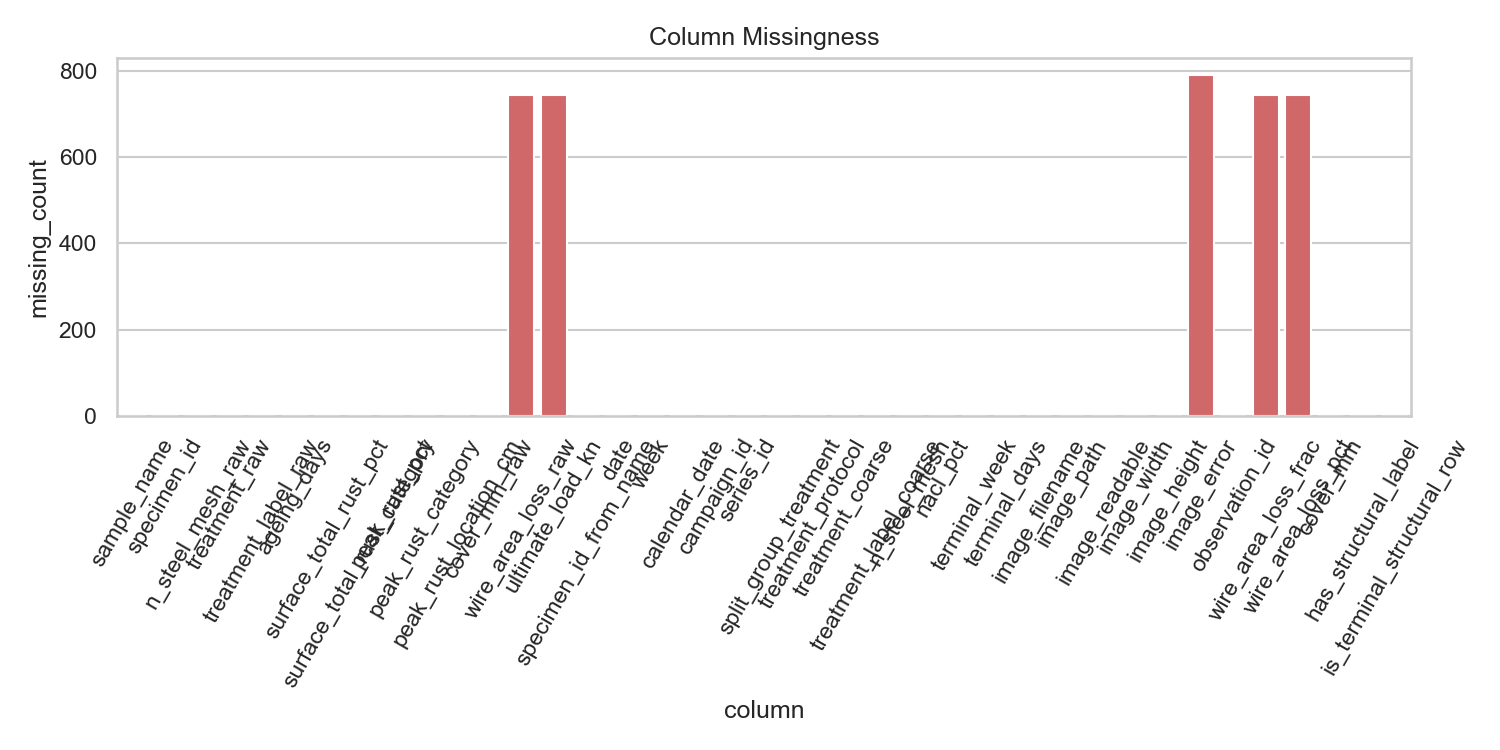
\includegraphics[width=0.88\textwidth]{outputs/eda/figures/missingness.png}
    \caption{Overall missingness structure in the aligned dataset. Surface variables are dense, while structural variables are sparse and terminal-only.}
    \label{fig:missingness}
\end{figure*}

\textbf{Interpretation and evidence strength.} Figure~\ref{fig:missingness} is strong evidence because it directly shows that the dataset is rich for visible corrosion analysis but sparse for structural supervision. This is one of the clearest justifications for avoiding direct supervised RUL prediction.

\begin{figure*}[t]
    \centering
    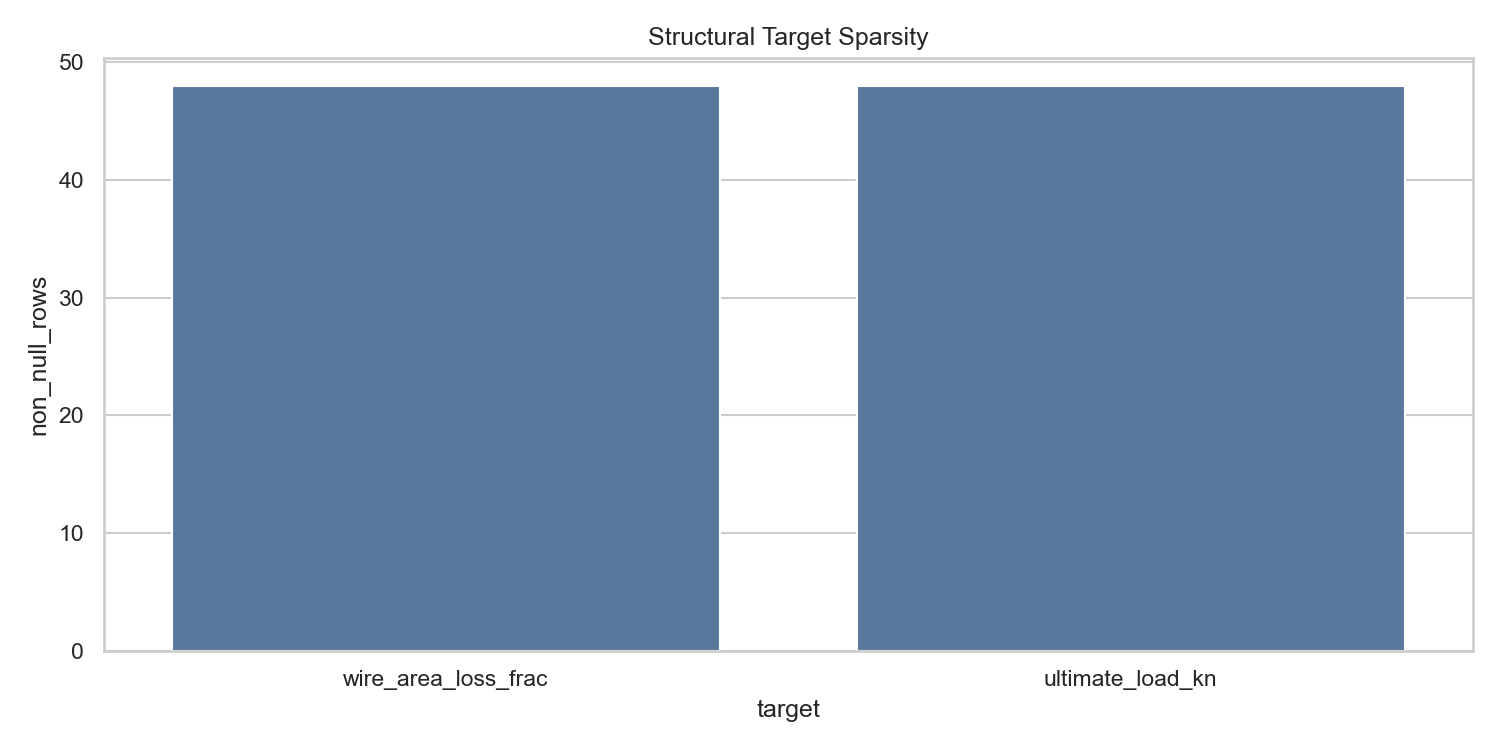
\includegraphics[width=0.82\textwidth]{outputs/eda/figures/structural_target_sparsity.png}
    \caption{Structural-label sparsity. Only one structural row per specimen is available, and those rows occur at terminal time points.}
    \label{fig:structural-sparsity}
\end{figure*}

\textbf{Interpretation and evidence strength.} Figure~\ref{fig:structural-sparsity} is also strong evidence. It supports the report's central formulation: visible corrosion can be studied densely, but hidden damage can only be studied through a small terminal subset.

\subsection{Feature distributions}

The feature-distribution diagnostics reveal a mixed picture:

\begin{itemize}
    \item many visible corrosion features have sensible broad ranges,
    \item some engineered features are strongly skewed,
    \item some features are effectively degenerate.
\end{itemize}

\subsection{Outliers}

The project deliberately kept outliers visible and added readability-focused views rather than hiding them. Figure~\ref{fig:trimmed-hists} shows selected skewed variables with plotting truncated at the 99th percentile for readability only.

\begin{figure*}[t]
    \centering
    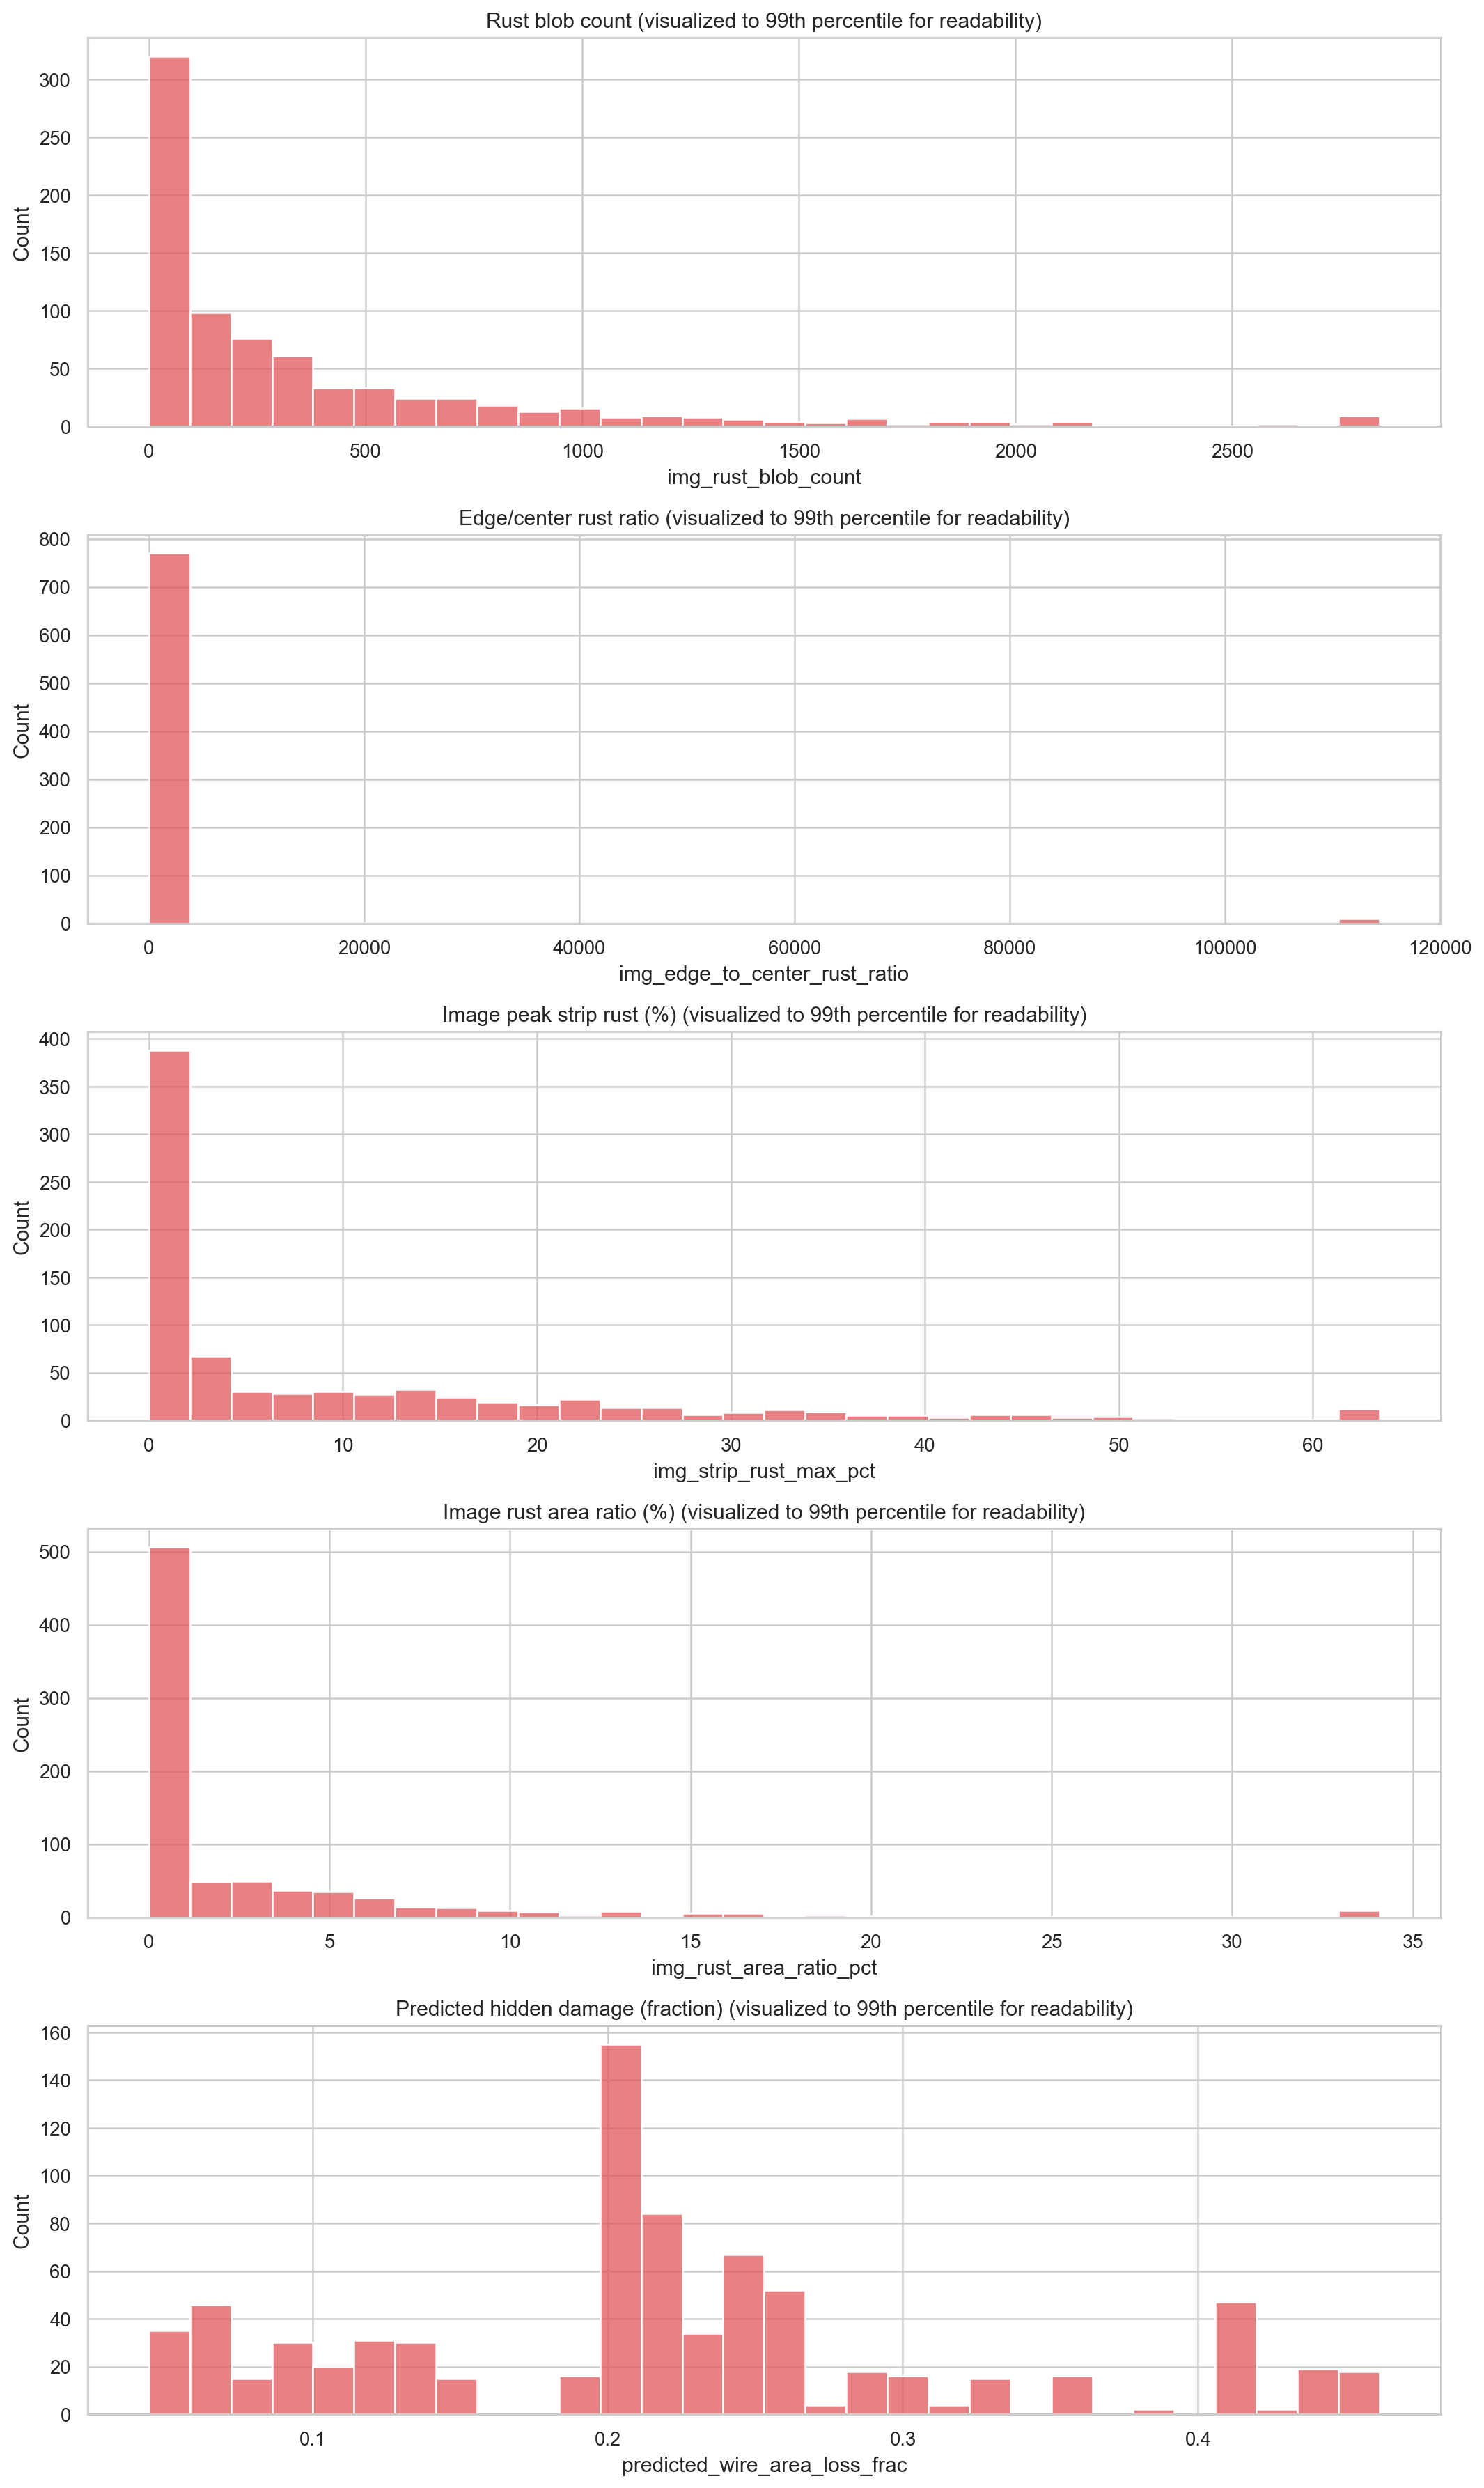
\includegraphics[width=0.93\textwidth]{outputs/diagnostics/figures/distributions/skewed_variable_histograms_trimmed_p99.png}
    \caption{Readability-focused histograms for heavily skewed variables. The plotting range is truncated at the 99th percentile for visibility, while full-range statistics are kept separately in the diagnostics tables.}
    \label{fig:trimmed-hists}
\end{figure*}

\textbf{Interpretation and evidence strength.} Figure~\ref{fig:trimmed-hists} is strong evidence for the claim that the feature space contains heavy tails and unstable engineered variables. This is especially important for explaining why feature cleanup was not cosmetic.

\subsection{Temporal progression}

Visible corrosion progression is one of the most meaningful parts of the dataset. Figure~\ref{fig:campaign-progress} shows the campaign-level progression summary, while Figure~\ref{fig:specimen-panels} shows representative specimen trajectories.

\begin{figure*}[t]
    \centering
    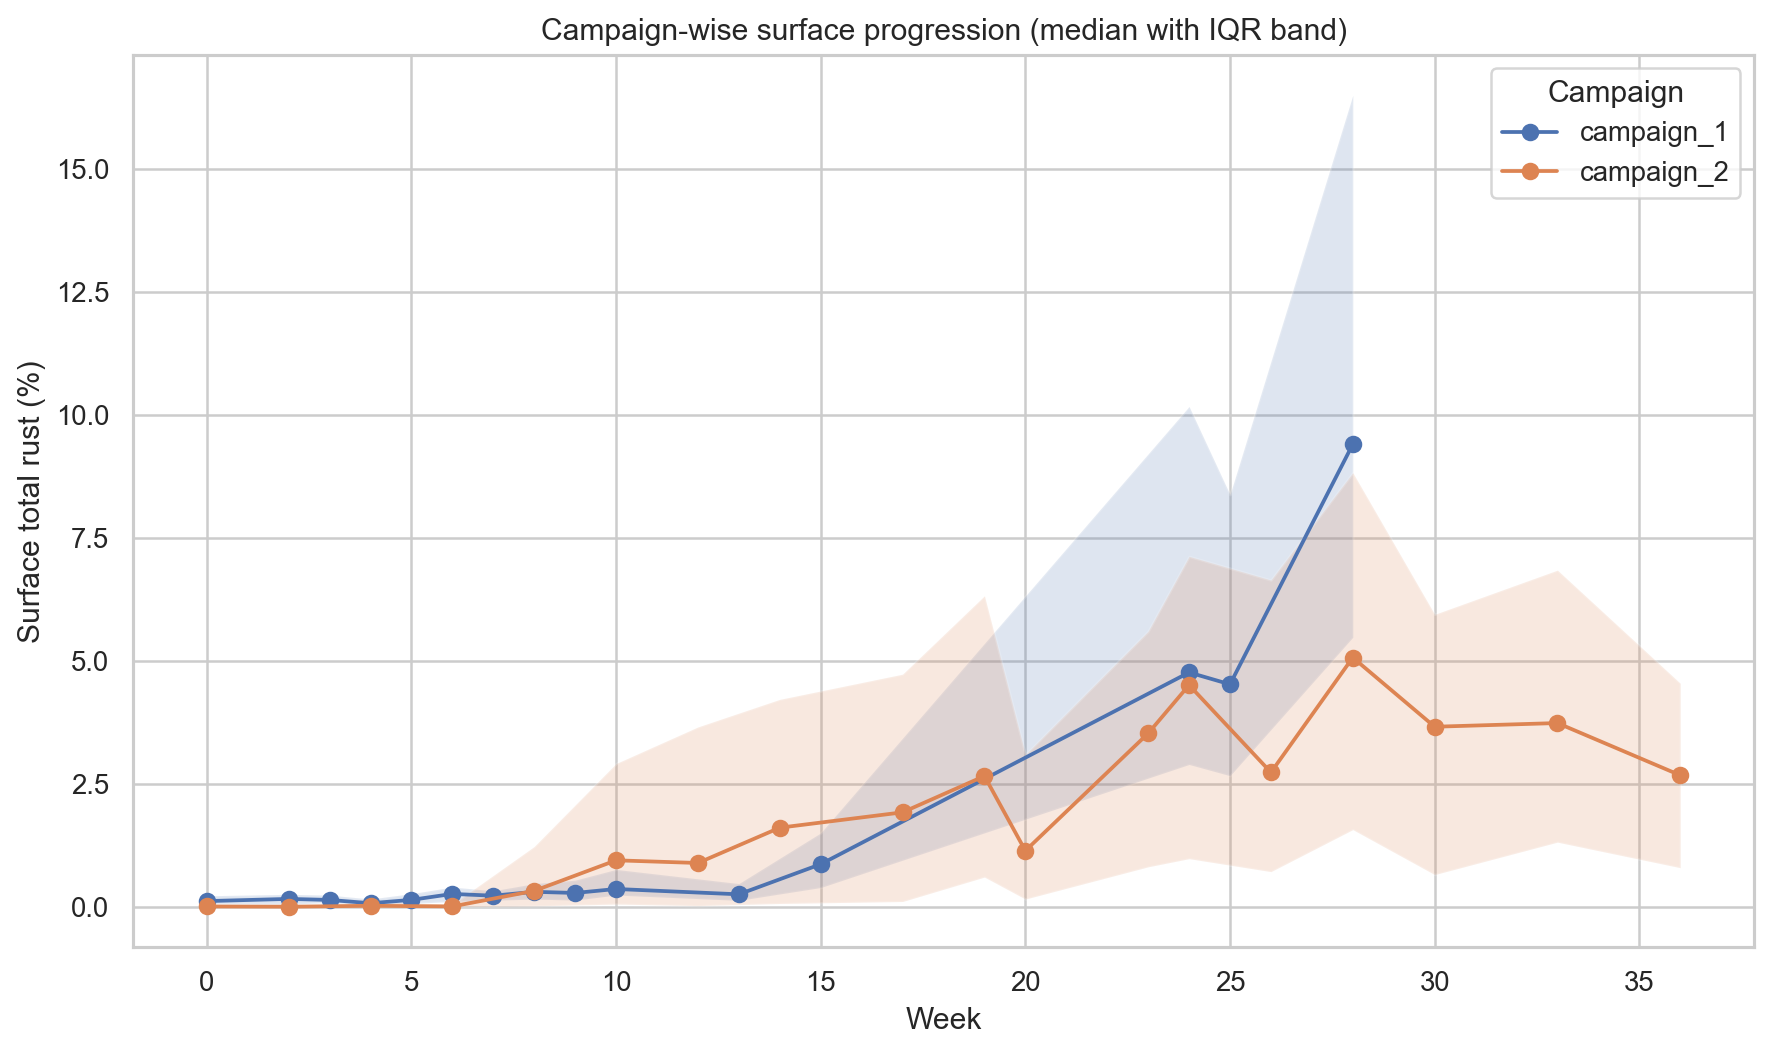
\includegraphics[width=0.9\textwidth]{outputs/diagnostics/figures/temporal/campaign_surface_progression_median_iqr.png}
    \caption{Campaign-level visible corrosion progression over time, shown as median behaviour with spread.}
    \label{fig:campaign-progress}
\end{figure*}

\textbf{Interpretation and evidence strength.} Figure~\ref{fig:campaign-progress} is strong evidence. It shows that visible corrosion generally increases with exposure time and that the two campaigns differ in both magnitude and spread. This is one of the most informative summary figures in the project.

\begin{figure*}[t]
    \centering
    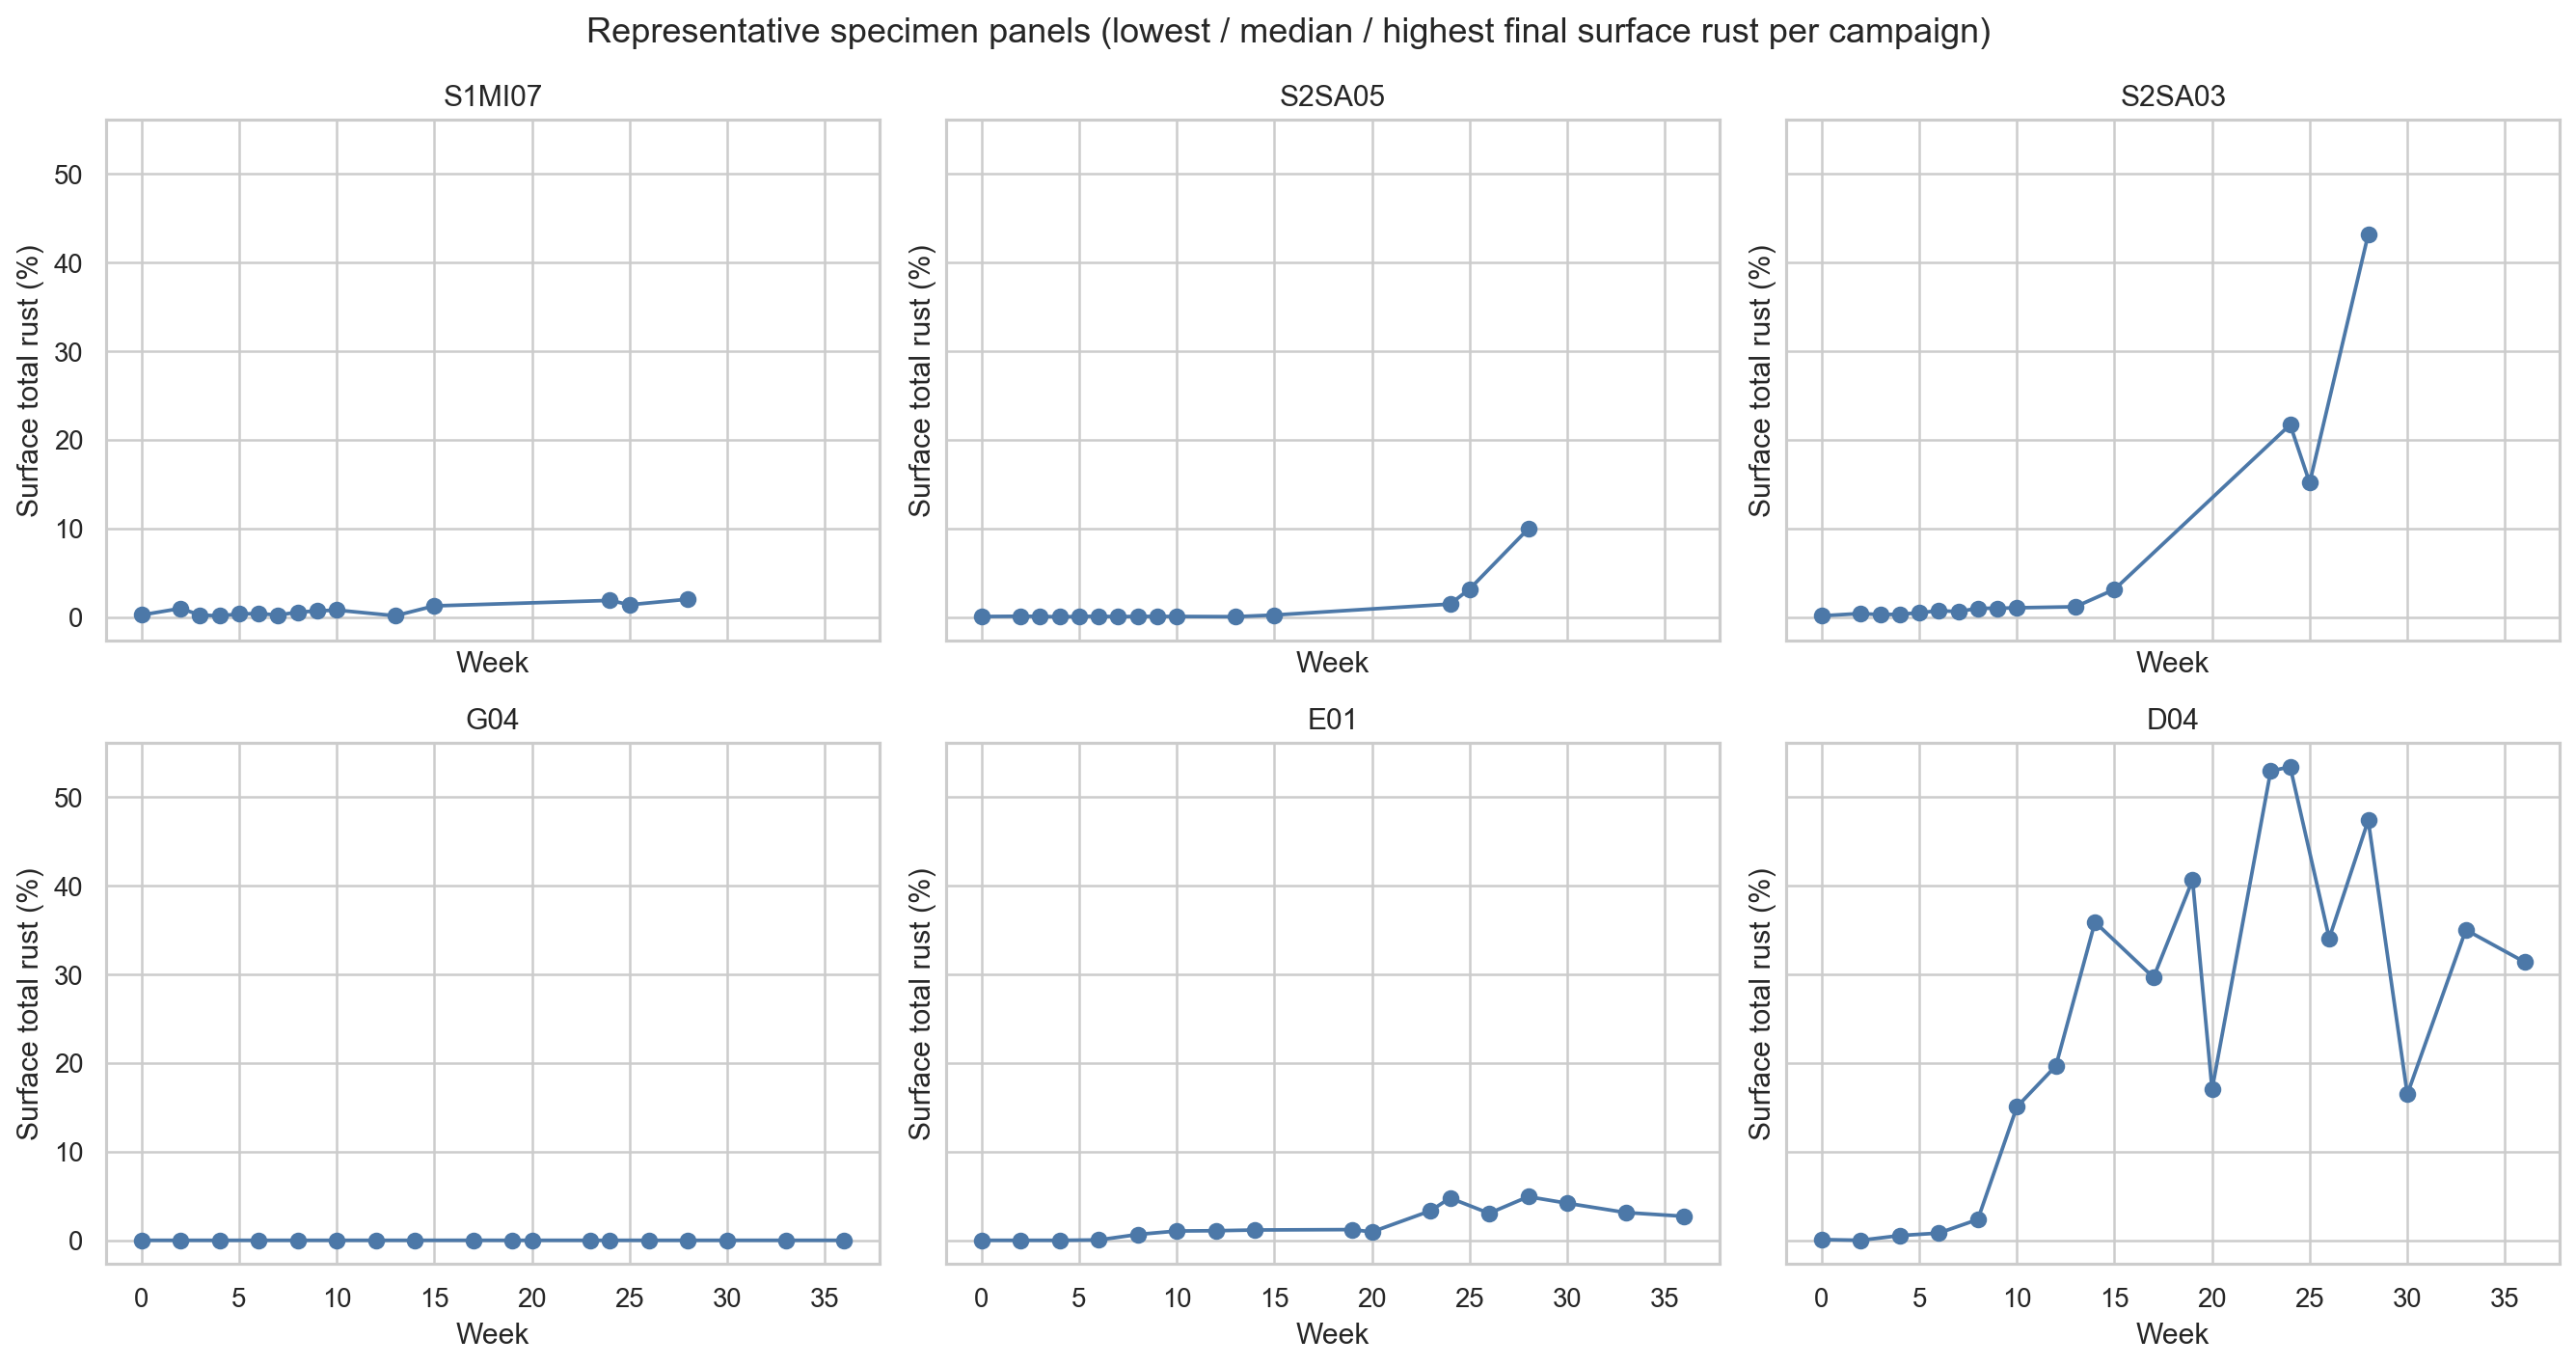
\includegraphics[width=0.9\textwidth]{outputs/diagnostics/figures/temporal/representative_specimen_surface_panels.png}
    \caption{Representative specimen-level surface corrosion trajectories.}
    \label{fig:specimen-panels}
\end{figure*}

\textbf{Interpretation and evidence strength.} Figure~\ref{fig:specimen-panels} is strong evidence because it makes the longitudinal nature of the dataset concrete. It also shows that specimen trajectories are informative but not perfectly smooth, which is important when later discussing degradation smoothing.

\begin{figure*}[t]
    \centering
    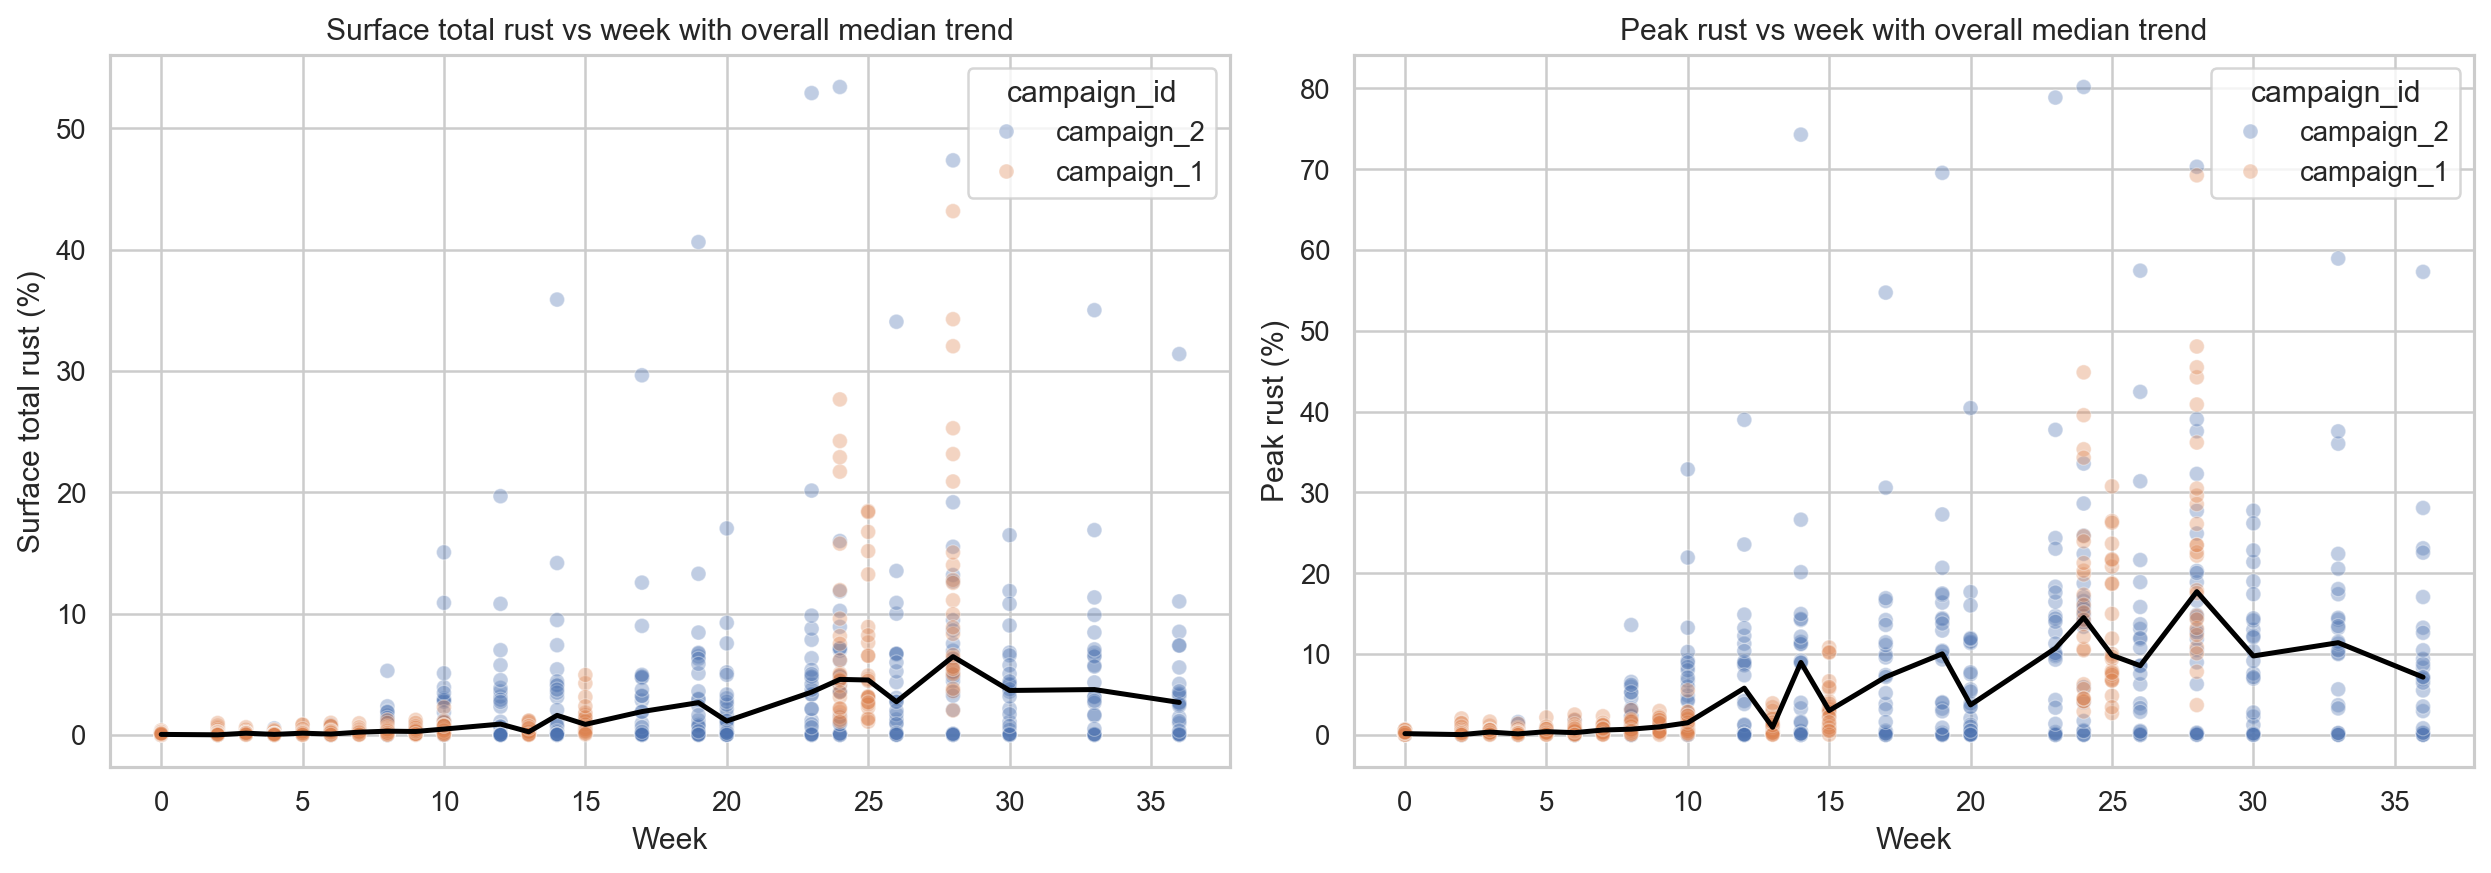
\includegraphics[width=0.9\textwidth]{outputs/diagnostics/figures/temporal/surface_progression_scatter_trends.png}
    \caption{Global scatter-and-trend view of visible corrosion progression over time.}
    \label{fig:scatter-trends}
\end{figure*}

\textbf{Interpretation and evidence strength.} Figure~\ref{fig:scatter-trends} is strong evidence for the existence of a broad upward corrosion trend. It is especially useful when a single figure is needed to summarize progression without focusing on individual specimens.

\subsection{Feature correlations}

Figure~\ref{fig:feature-target-corr} shows the focused feature-target correlation heatmap. This is one of the most important figures in the entire project because it clarifies what the engineered features actually capture.

\begin{figure*}[t]
    \centering
    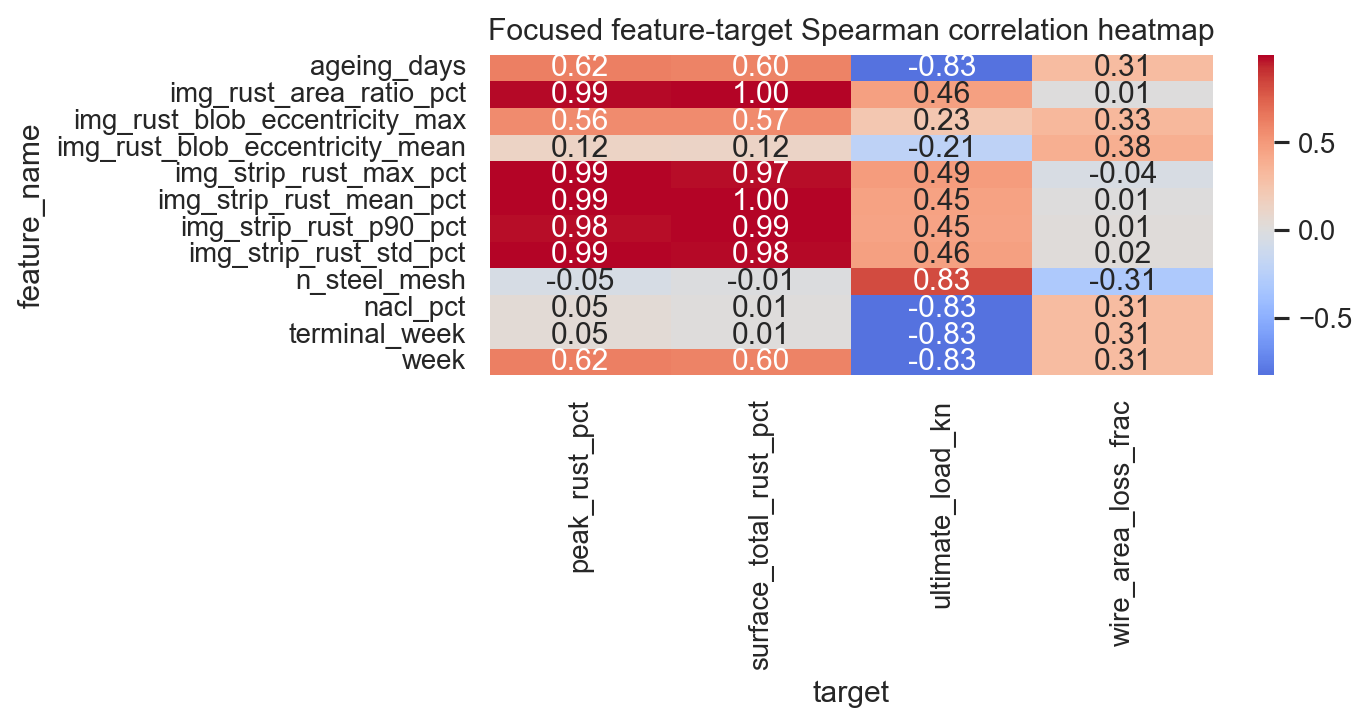
\includegraphics[width=0.93\textwidth]{outputs/diagnostics/figures/features/feature_target_correlation_heatmap.png}
    \caption{Focused feature-target correlation heatmap for visible corrosion targets and sparse structural targets.}
    \label{fig:feature-target-corr}
\end{figure*}

\textbf{Interpretation and evidence strength.} Figure~\ref{fig:feature-target-corr} is strong evidence. It shows that the engineered image features track visible corrosion very strongly, especially for \texttt{surface\_total\_rust\_pct} and \texttt{peak\_rust\_pct}, but that the relationship to sparse structural targets is much weaker. The strongest univariate correlation with \texttt{wire\_area\_loss\_frac} is only about 0.38, which already signals a hard hidden-damage problem before model fitting begins.

\subsection{Redundancy and collinearity}

Two complementary figures explain redundancy. Figure~\ref{fig:image-corr} shows the correlation structure among key image features. Figure~\ref{fig:collinearity} shows the highest-collinearity feature pairs that motivated explicit cleanup.

\begin{figure*}[t]
    \centering
    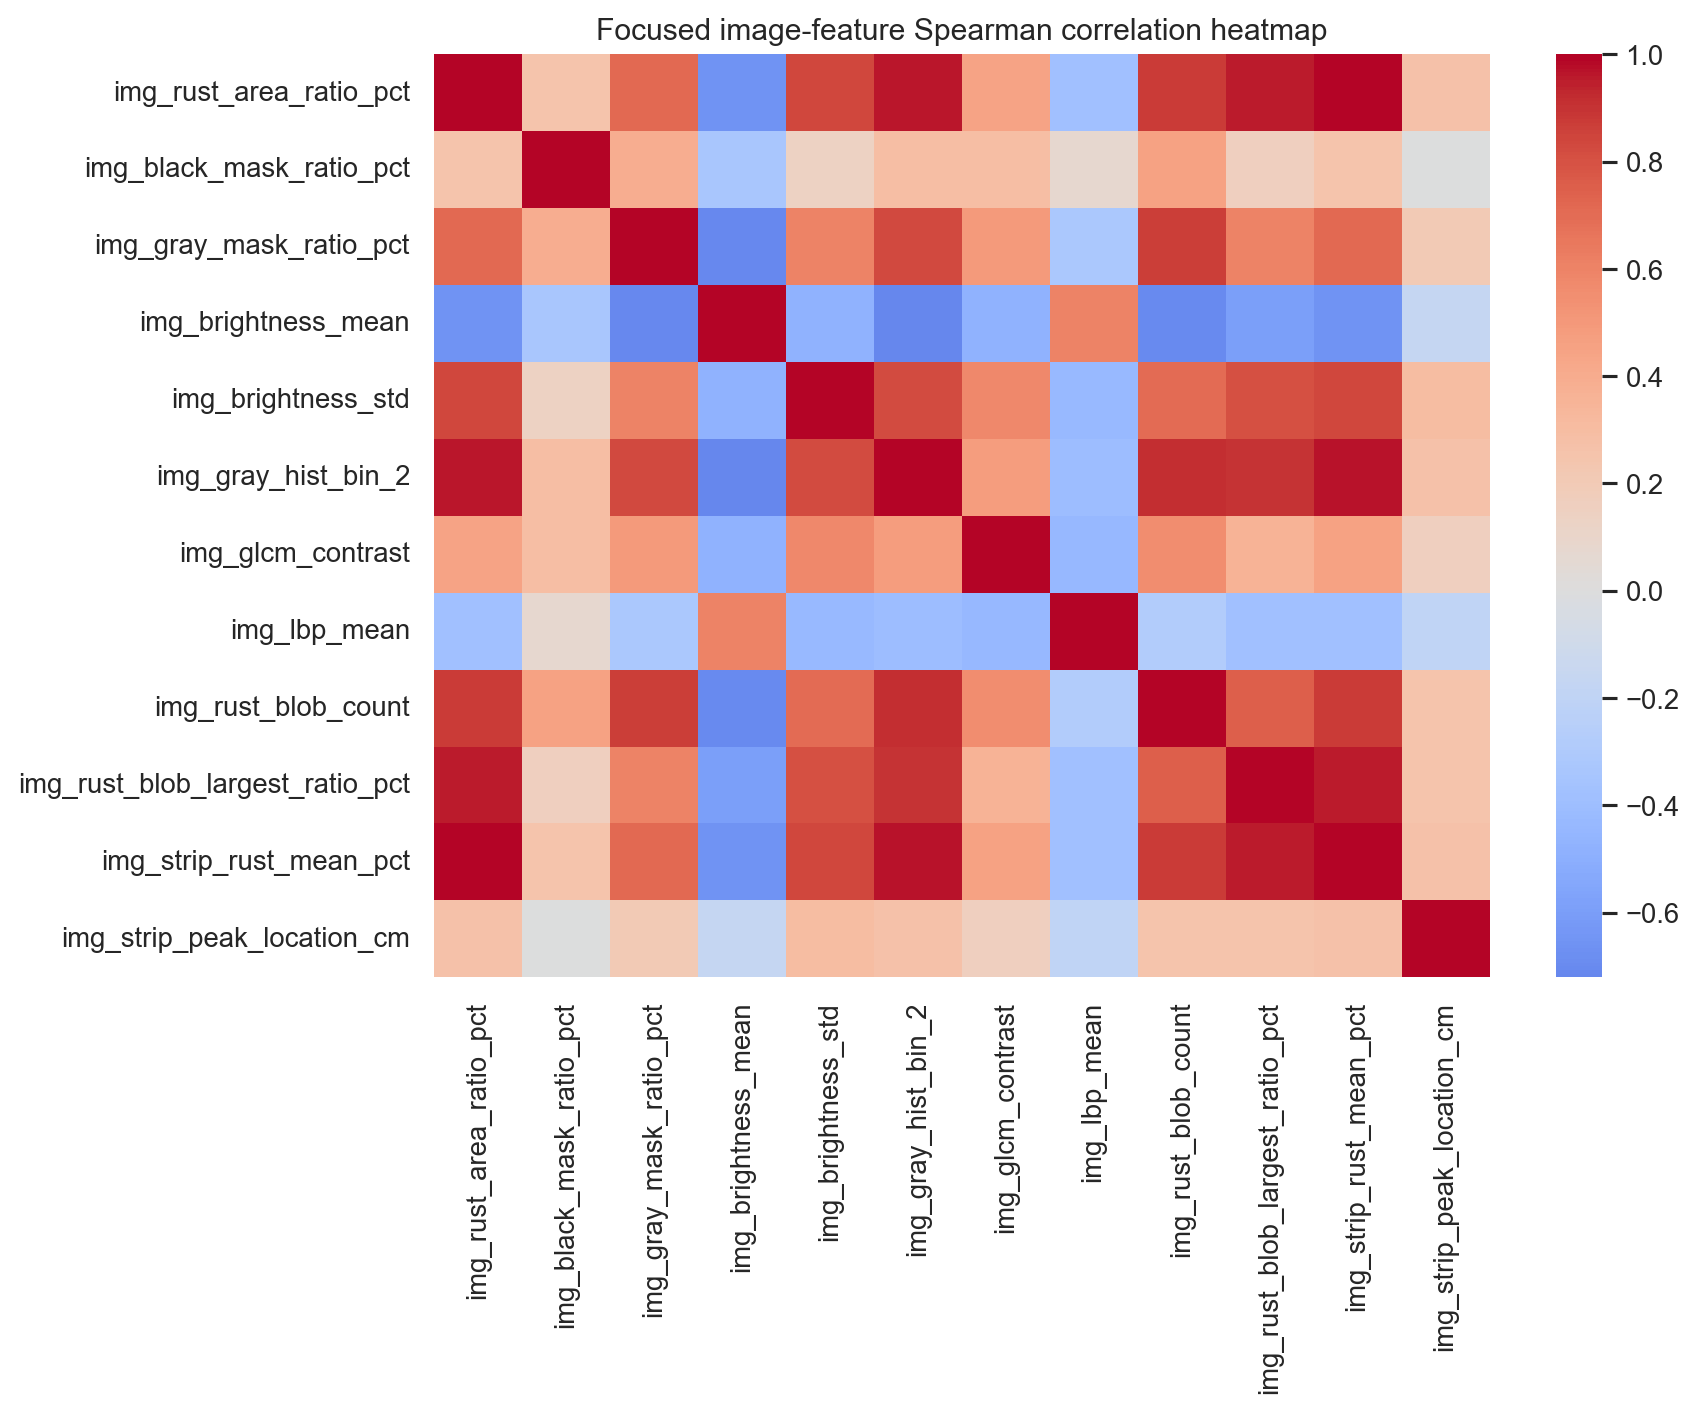
\includegraphics[width=0.85\textwidth]{outputs/diagnostics/figures/features/image_feature_correlation_heatmap.png}
    \caption{Correlation heatmap for key image features. Many features move together because they describe related aspects of visible corrosion.}
    \label{fig:image-corr}
\end{figure*}

\textbf{Interpretation and evidence strength.} Figure~\ref{fig:image-corr} is strong evidence that the feature space is not a collection of independent signals. Several image-derived features reflect the same underlying corrosion pattern, which helps explain why feature cleanup and family-based interpretation are necessary.

\begin{figure*}[t]
    \centering
    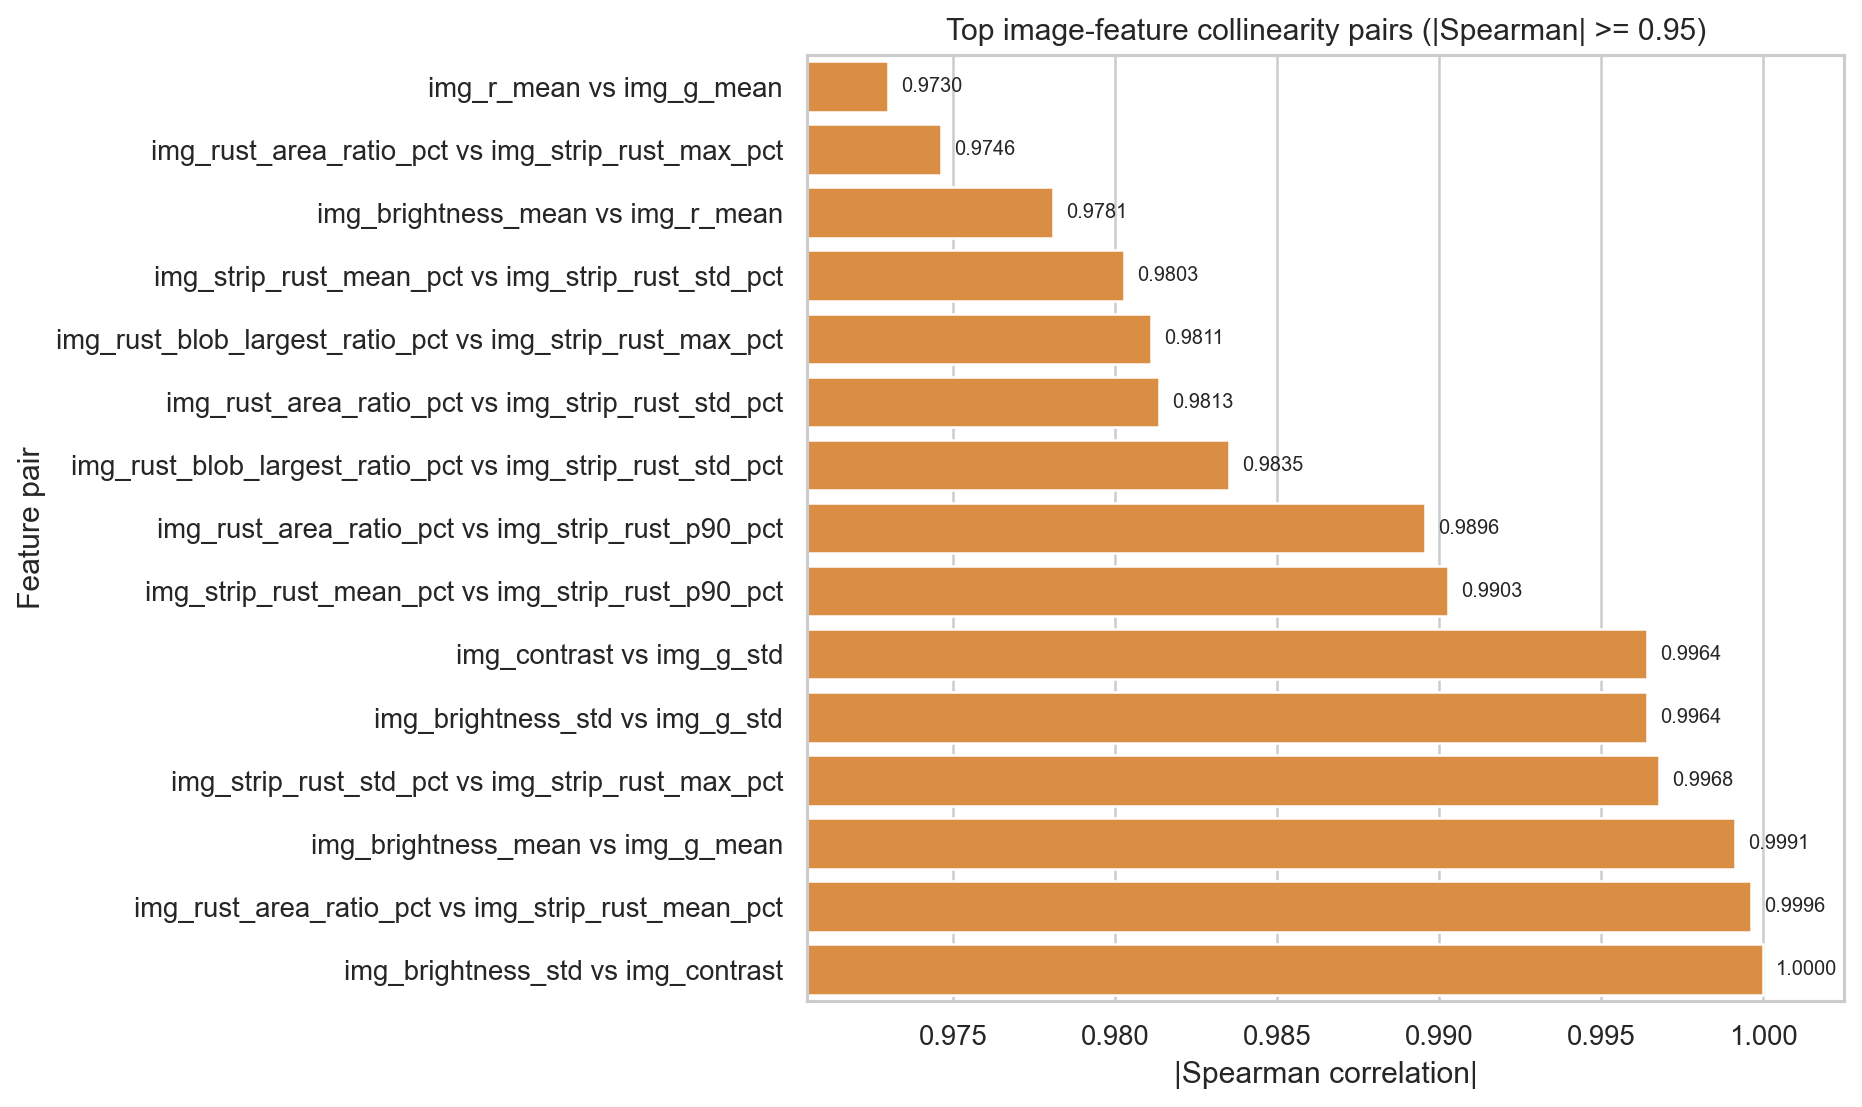
\includegraphics[width=0.88\textwidth]{outputs/diagnostics/figures/features/high_collinearity_pairs.png}
    \caption{Highest-collinearity feature pairs found during diagnostics.}
    \label{fig:collinearity}
\end{figure*}

\textbf{Interpretation and evidence strength.} Figure~\ref{fig:collinearity} is strong evidence that redundancy is a real modelling issue, not a cosmetic concern. The diagnostics found many highly collinear pairs, in addition to exact duplicates and near-constant features. This makes the later feature-space cleanup scientifically well motivated.

\section{Model Benchmarking and Results}

\subsection{Grouped split results}

The grouped split results provide the baseline within-dataset evaluation. The main grouped findings are:

\begin{itemize}
    \item the surface stage performs strongly, but its main target is partly tautological,
    \item \texttt{peak\_rust\_pct} remains a useful auxiliary surface benchmark,
    \item the hidden-damage stage is much weaker, especially for \texttt{wire\_area\_loss\_frac}.
\end{itemize}

Two grouped facts are particularly important:

\begin{itemize}
    \item the extracted rust-area feature reconstructs \texttt{surface\_total\_rust\_pct} almost exactly, with MAE 0.000228 and maximum absolute difference below 0.000500,
    \item the selected final hidden-damage models use only 8 metadata features for each structural target.
\end{itemize}

\subsection{Leave-one-treatment-out}

Leave-one-treatment-out is a harder test than grouped holdout because it asks whether a learned pattern transfers across treatment groups. For the current selected structural models:

\begin{itemize}
    \item \texttt{wire\_area\_loss\_frac}: MAE 0.116 and Spearman 0.186,
    \item \texttt{ultimate\_load\_kn}: MAE 0.203 and Spearman 0.122.
\end{itemize}

These values are not strong enough to claim reliable structural generalization, but they are still more informative than the grouped split alone.

\subsection{Leave-one-campaign-out}

Leave-one-campaign-out is the most scientifically important evaluation regime because it tests a real shift in experimental setting. It is also where the structural stage remains weakest.

For the final robustness-selected structural models:

\begin{itemize}
    \item \texttt{wire\_area\_loss\_frac}: MAE 0.121, Spearman -0.266,
    \item \texttt{ultimate\_load\_kn}: MAE 0.564, Spearman 0.353.
\end{itemize}

These results show that the project still does not support strong cross-campaign hidden-damage claims.

\subsection{Robustness discussion}

Benchmark robustness matters more than a single best grouped score because the grouped split is the easiest regime. Figure~\ref{fig:collapse-heatmap} summarizes how error changes when the split becomes harder.

\begin{figure*}[t]
    \centering
    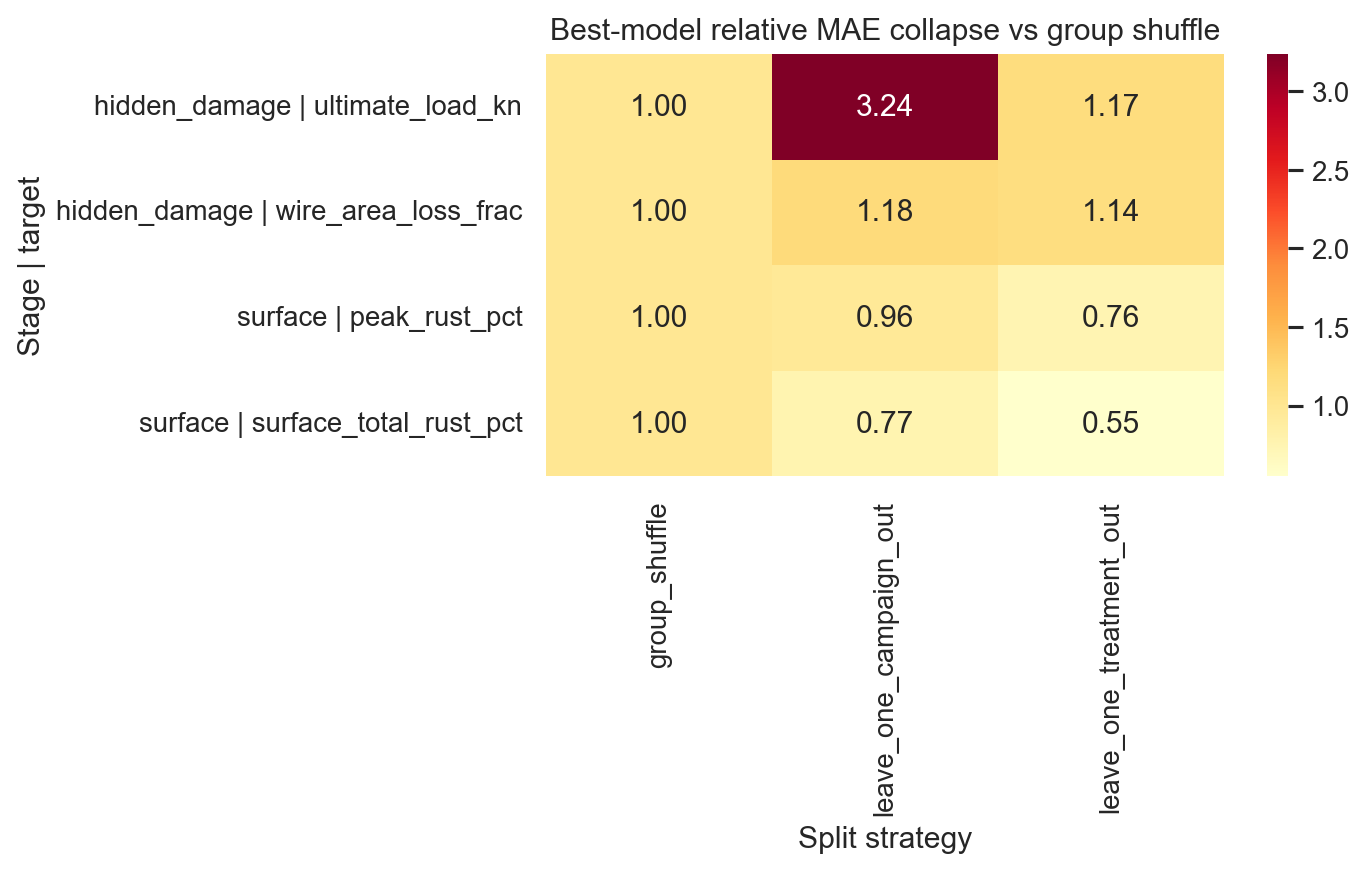
\includegraphics[width=0.88\textwidth]{outputs/diagnostics/figures/benchmarks/best_model_relative_mae_collapse_heatmap.png}
    \caption{Relative MAE collapse across split strategies. Values above 1 indicate worse performance than the grouped baseline.}
    \label{fig:collapse-heatmap}
\end{figure*}

\textbf{Interpretation and evidence strength.} Figure~\ref{fig:collapse-heatmap} is strong evidence because it summarizes the central robustness lesson of the project. Surface benchmarks remain relatively stable, while structural benchmarks deteriorate markedly under harder evaluation.

Figure~\ref{fig:hidden-robustness} complements that view by showing the structural best-model robustness directly.

\begin{figure*}[t]
    \centering
    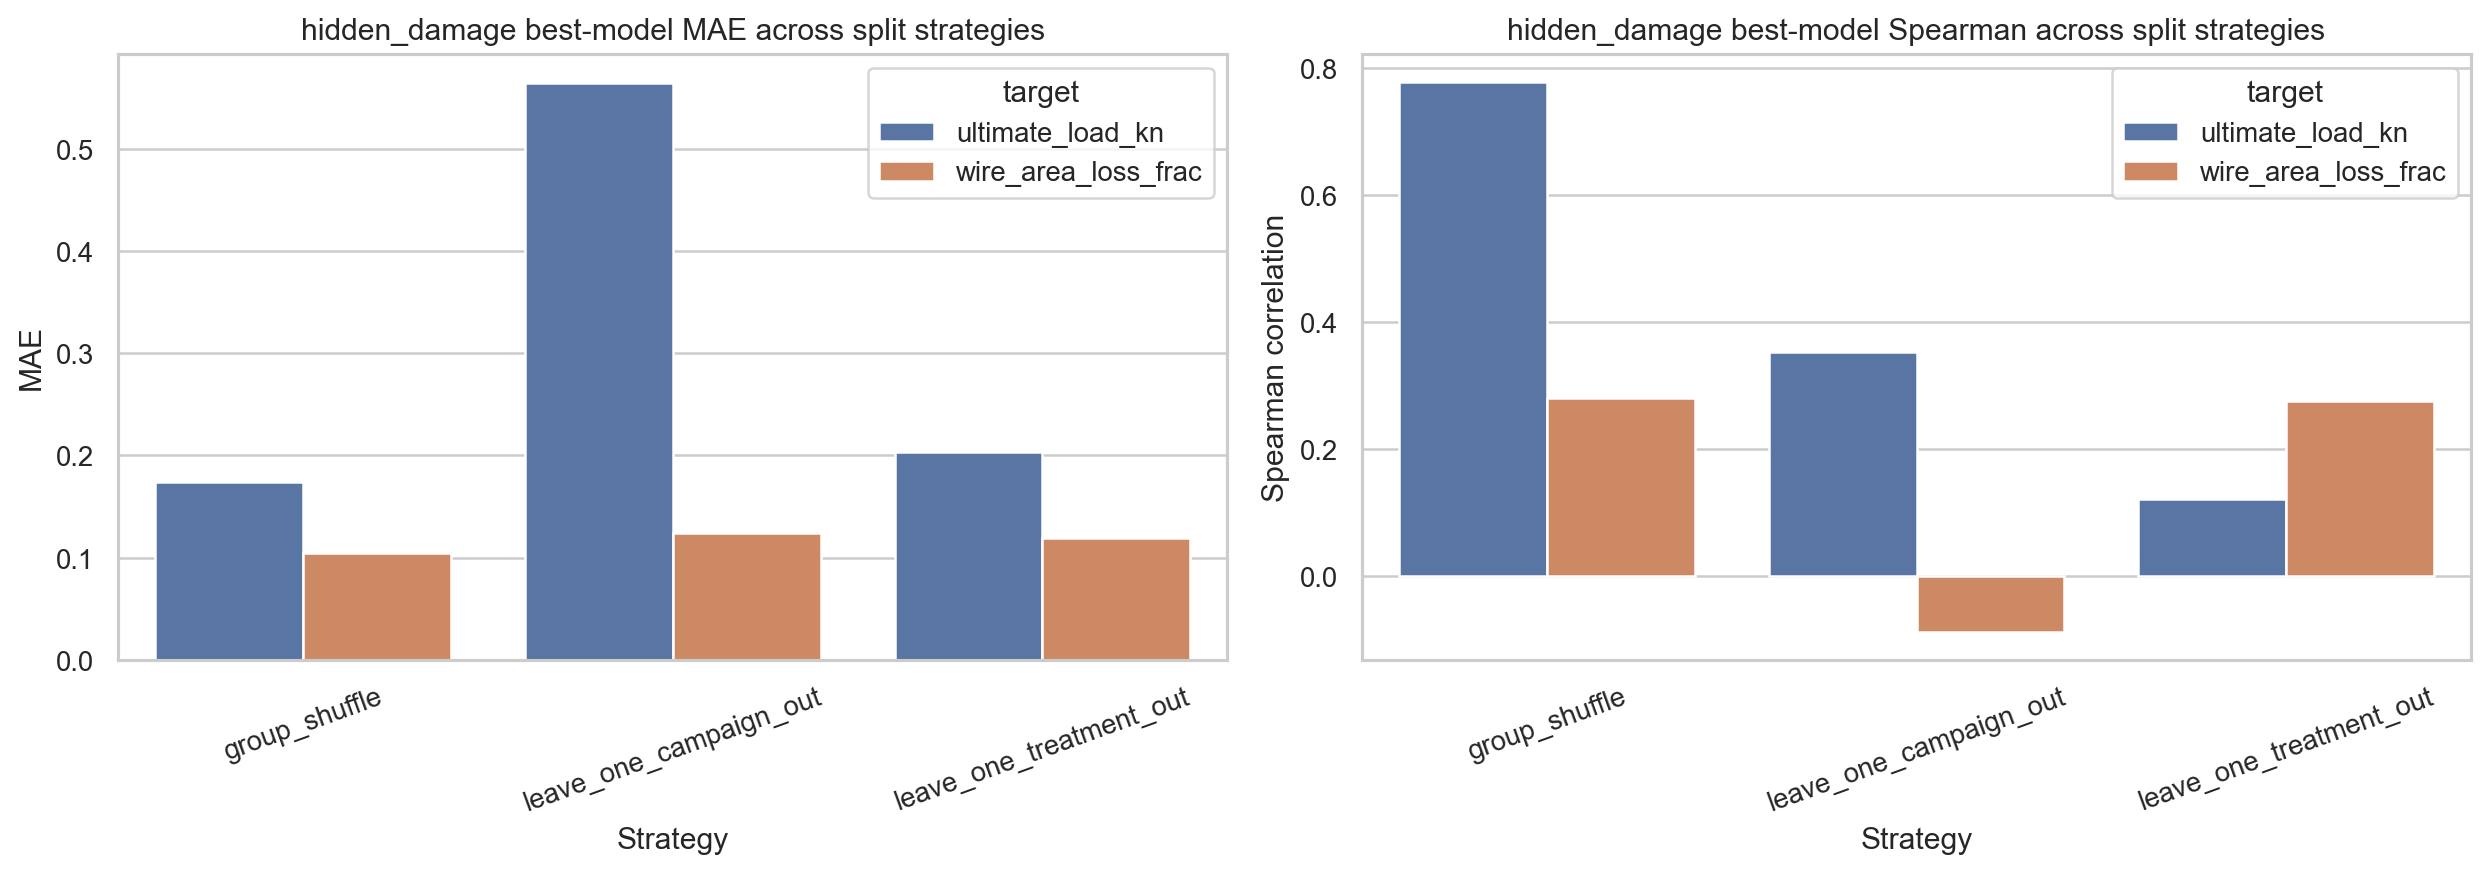
\includegraphics[width=0.88\textwidth]{outputs/diagnostics/figures/benchmarks/hidden_damage_best_model_strategy_robustness.png}
    \caption{Robustness profile of the selected structural models across grouped, leave-one-treatment-out, and leave-one-campaign-out evaluation.}
    \label{fig:hidden-robustness}
\end{figure*}

\textbf{Interpretation and evidence strength.} Figure~\ref{fig:hidden-robustness} is strong evidence. It shows clearly that structural modelling is the weak part of the pipeline, and it also supports the conclusion that benchmark robustness is a better guide than one good average score.

Table~\ref{tab:benchmark-snapshot} summarizes the current benchmark snapshot after feature cleanup and robustness-aware model selection.

\begin{table*}[t]
\centering
\caption{Current benchmark snapshot for the most relevant targets. The structural rows correspond to the final robustness-selected models.}
\label{tab:benchmark-snapshot}
\small
\begin{tabularx}{\textwidth}{p{0.17\textwidth}p{0.17\textwidth}p{0.12\textwidth}Y}
\toprule
\textbf{Target} & \textbf{Current model / feature set} & \textbf{Key metrics} & \textbf{Interpretation} \\
\midrule
\texttt{surface\_total\_rust\_pct} & rust-area reconstruction sanity check & MAE 0.000228, Spearman 0.9996 between label and extracted rust area & Strong as pipeline validation, but not a substantive hidden-damage result. \\
\texttt{peak\_rust\_pct} & Random Forest / full surface feature table & Grouped MAE 1.097, grouped Spearman 0.992, LOCO MAE 1.058, LOCO Spearman 0.977 & Meaningful auxiliary visible-corrosion benchmark. \\
\texttt{wire\_area\_loss\_frac} & CatBoost / metadata-only & Grouped MAE 0.124, grouped Spearman 0.289, LOCO MAE 0.121, LOCO Spearman -0.266 & Weak and unstable. Better viewed as a difficult negative result than as a predictive success. \\
\texttt{ultimate\_load\_kn} & Random Forest / metadata-only & Grouped MAE 0.174, grouped Spearman 0.778, LOCO MAE 0.564, LOCO Spearman 0.353 & Improved relative to the earlier baseline, but still too fragile for strong cross-campaign claims. \\
\bottomrule
\end{tabularx}
\end{table*}

The improvement round is still important to mention. Compared with the earlier baseline, leave-one-campaign-out absolute error improved for both structural targets, but the improvement was uneven:

\begin{itemize}
    \item \texttt{ultimate\_load\_kn} improved in a relatively clean way,
    \item \texttt{wire\_area\_loss\_frac} improved in MAE on the harder splits but remained weak in ranking and even worsened in leave-one-campaign-out Spearman.
\end{itemize}

\subsection{Degradation modelling}

The degradation stage should be interpreted conservatively. It smooths model-generated hidden-damage proxies over time. Figure~\ref{fig:degradation-raw-monotone} shows why this smoothing was introduced.

\begin{figure*}[t]
    \centering
    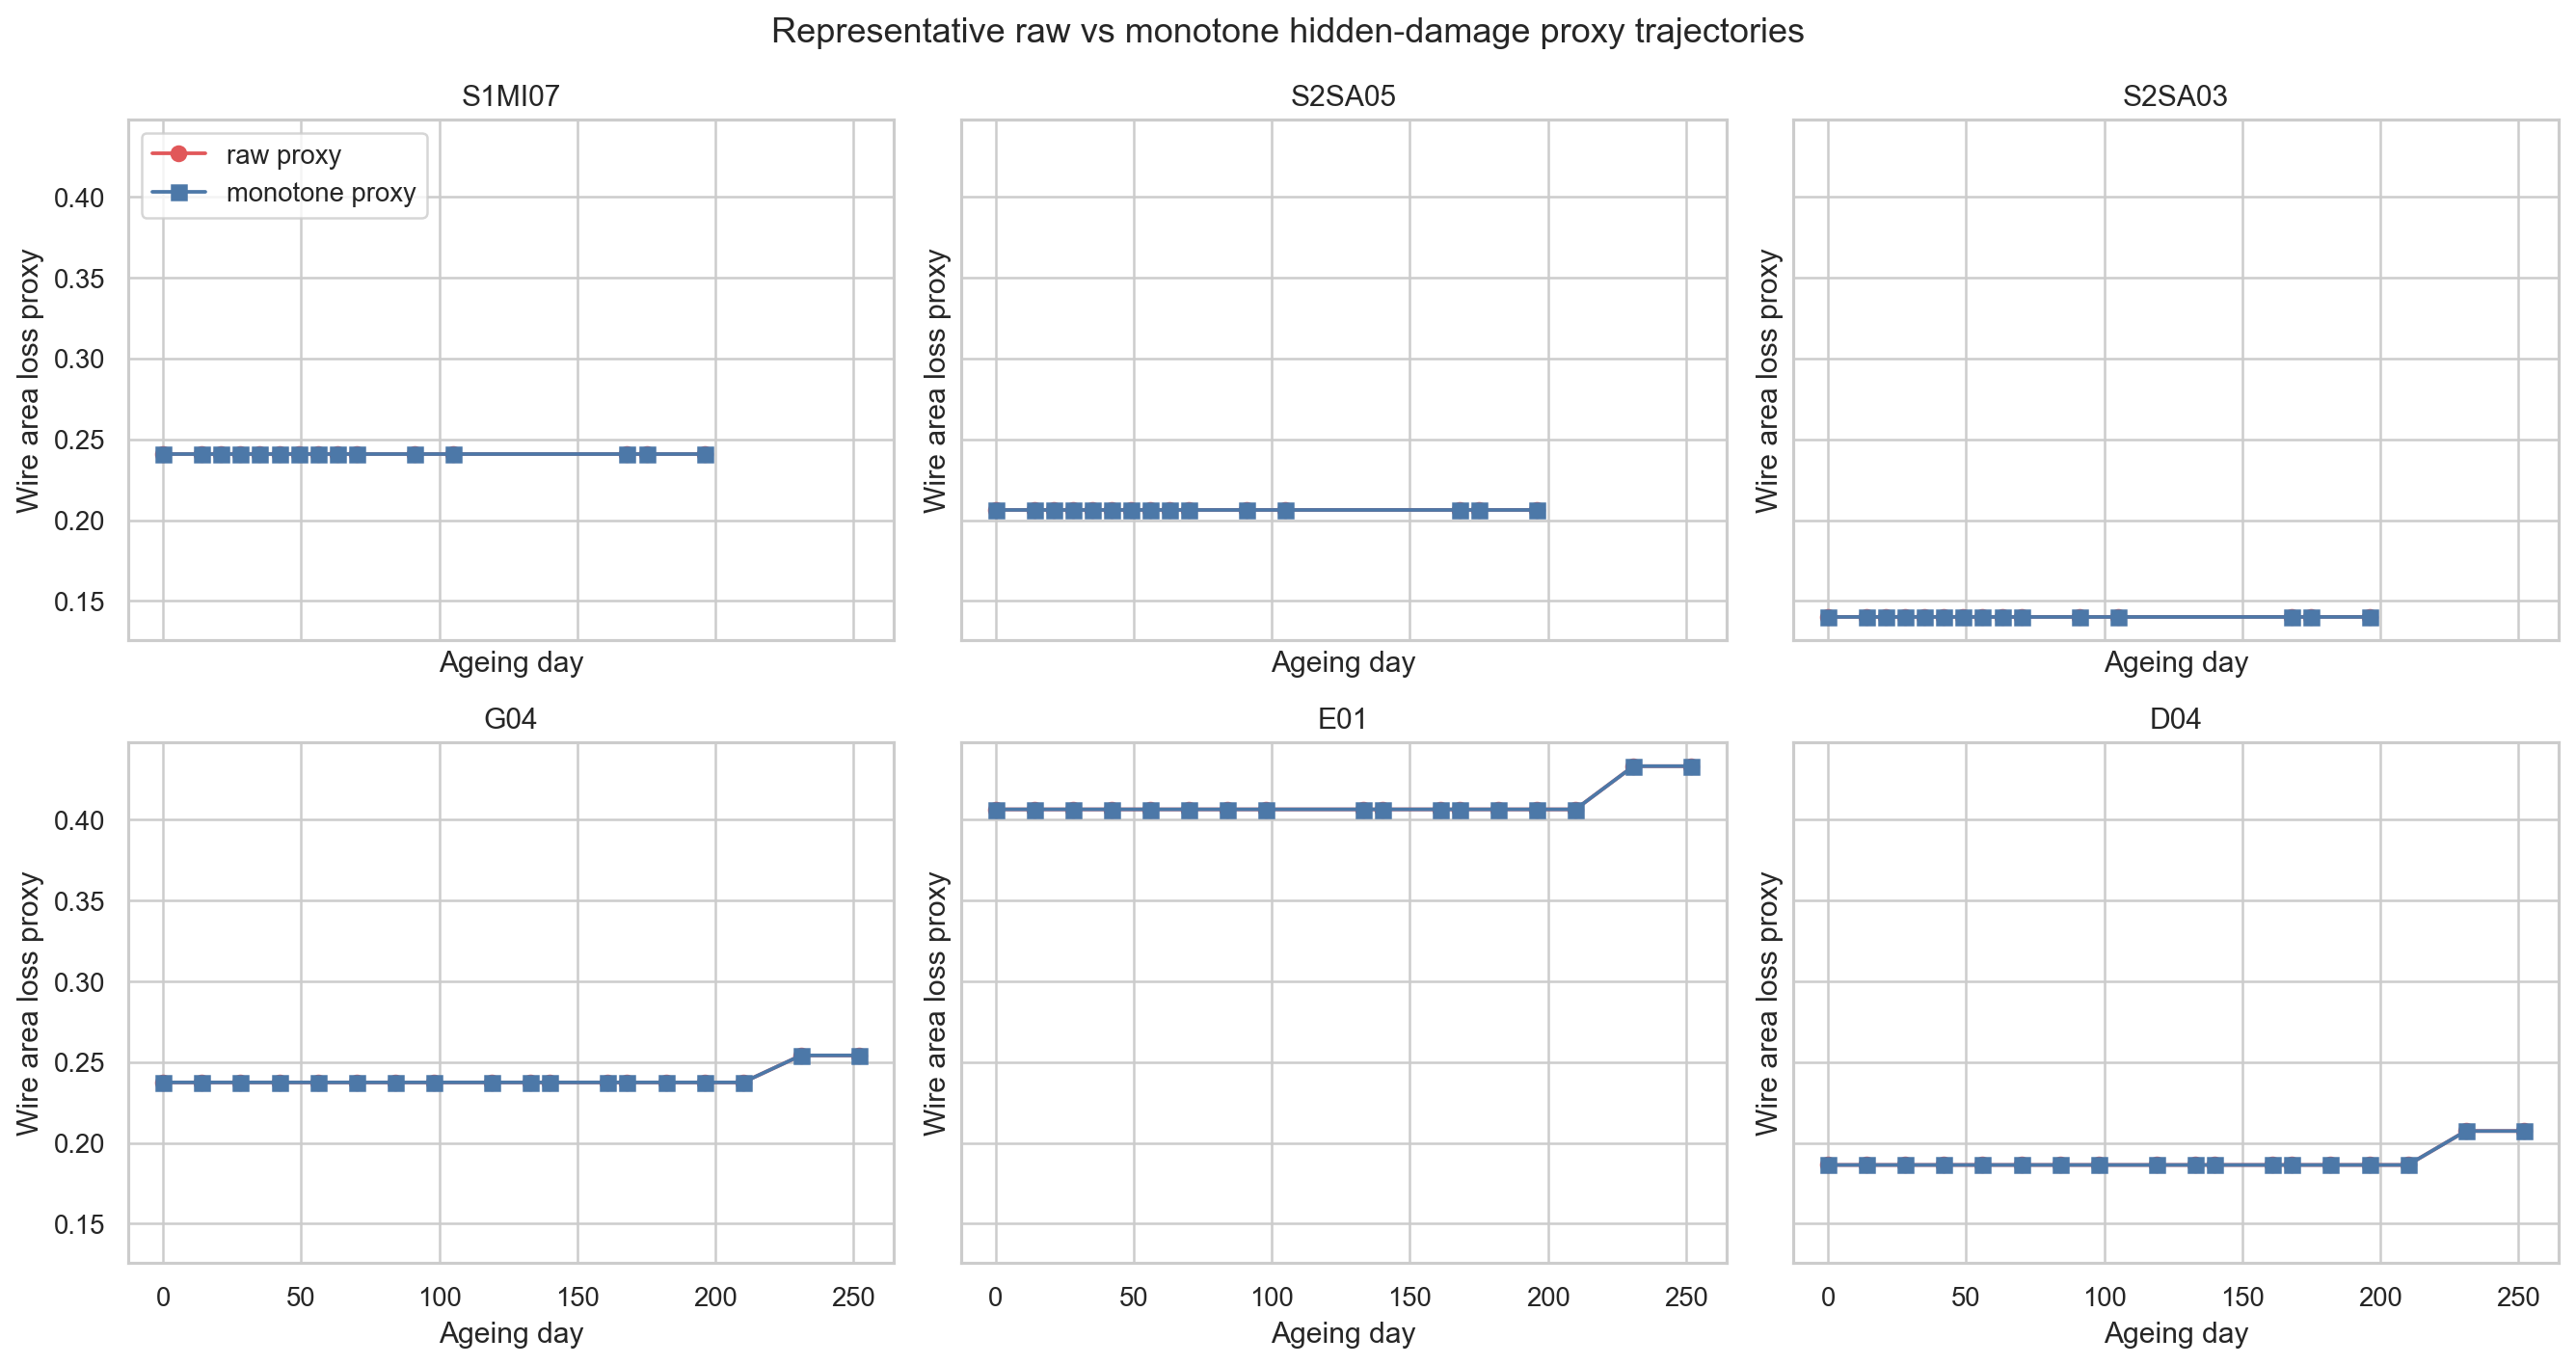
\includegraphics[width=0.88\textwidth]{outputs/diagnostics/figures/degradation/degradation_raw_vs_monotone_representative.png}
    \caption{Representative raw hidden-damage proxy trajectories compared with their monotone-smoothed versions.}
    \label{fig:degradation-raw-monotone}
\end{figure*}

\textbf{Interpretation and evidence strength.} Figure~\ref{fig:degradation-raw-monotone} is moderate evidence. It honestly shows that the degradation stage is primarily a stabilizing descriptive layer, added because the raw hidden-damage proxy is not cleanly monotone over time.

\subsection{Proxy-RUL logic}

The final proxy-RUL output is best interpreted as threshold-status analysis. Figure~\ref{fig:proxy-status} summarizes the current status.

\begin{figure*}[t]
    \centering
    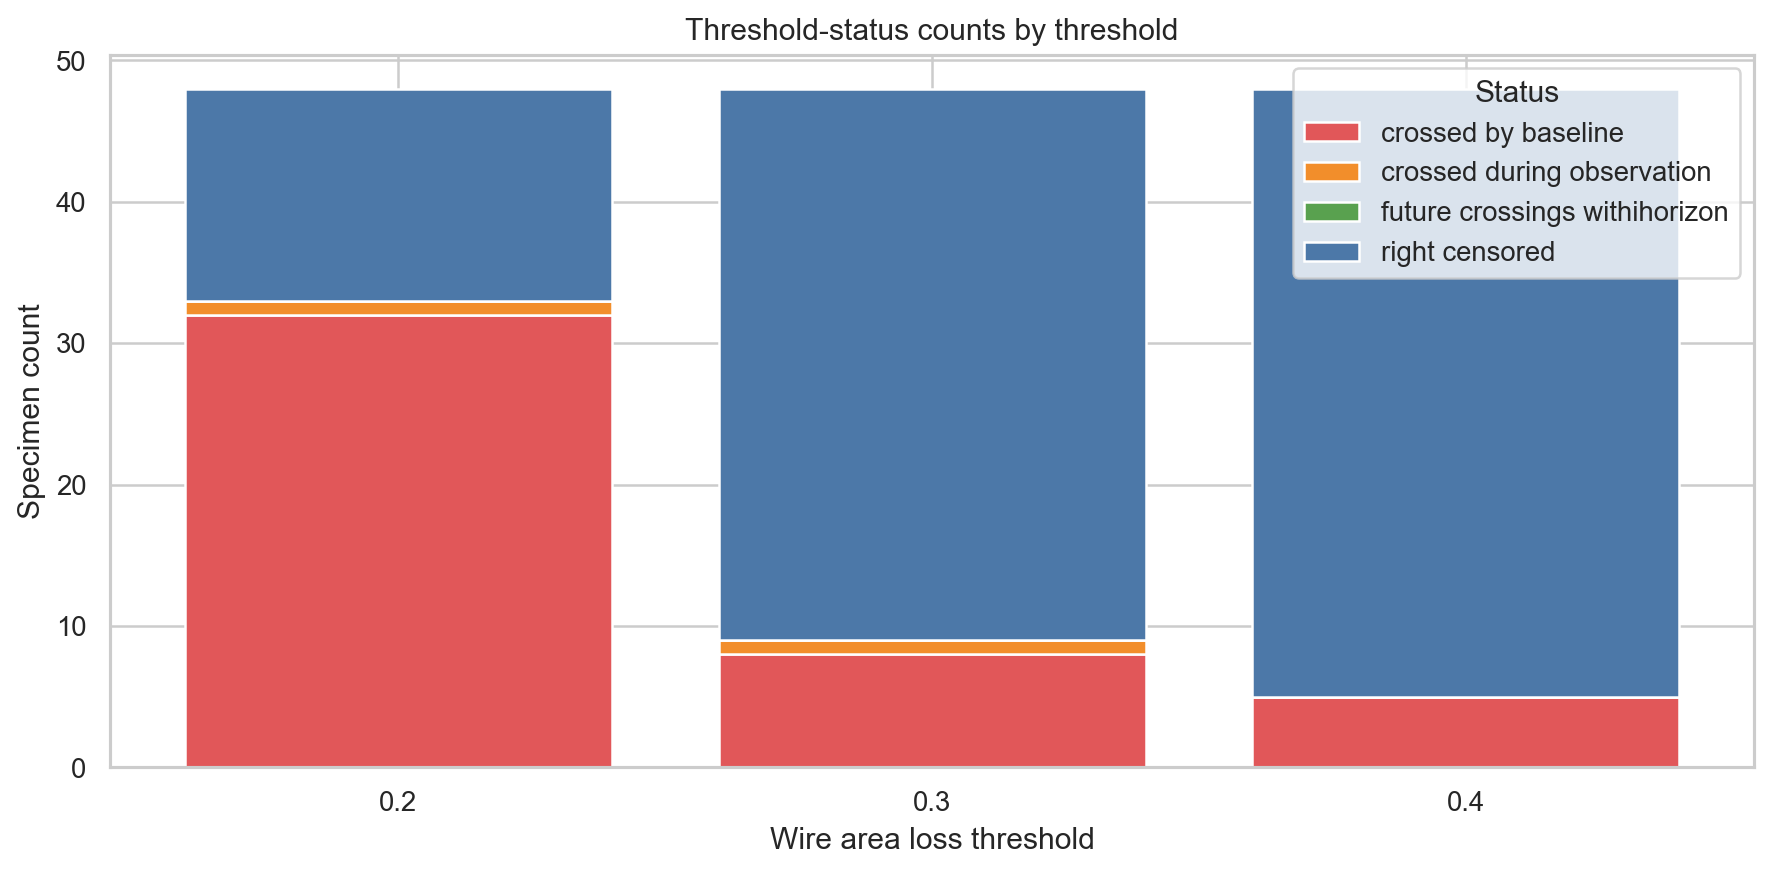
\includegraphics[width=0.88\textwidth]{outputs/diagnostics/figures/proxy/proxy_threshold_status_counts.png}
    \caption{Threshold-status counts for the proxy-RUL stage. Most cases are already crossed or right-censored, and no future threshold crossings occur within the projection horizon.}
    \label{fig:proxy-status}
\end{figure*}

\textbf{Interpretation and evidence strength.} Figure~\ref{fig:proxy-status} is strong as an honesty figure, but weak as predictive evidence. It matters because it makes the current state of the proxy-RUL stage very clear: the pipeline does not yet provide useful forward residual-life estimates.

\section{Important Figures and Their Interpretation}
\label{sec:important-figures}

This section compares the most meaningful figures and explains why they are more useful than some visually attractive alternatives.

\subsection{Figures that explain the dataset constraints}

Figures~\ref{fig:missingness} and \ref{fig:structural-sparsity} are the best pair for explaining the dataset limitation. The first figure shows the broad missingness structure; the second figure turns that into a direct structural-label message. Together they justify the entire staged formulation.

These figures are stronger than simple count charts such as row counts, campaign counts, or treatment counts because they explain not just \emph{how much} data exists, but \emph{what kind} of supervision is actually available.

\subsection{Figures that explain corrosion progression}

Figures~\ref{fig:campaign-progress}, \ref{fig:specimen-panels}, and \ref{fig:scatter-trends} work well as a sequence:

\begin{itemize}
    \item Figure~\ref{fig:campaign-progress} shows the campaign-level trend,
    \item Figure~\ref{fig:specimen-panels} shows representative specimen-level behaviour,
    \item Figure~\ref{fig:scatter-trends} shows the broad global relationship with time.
\end{itemize}

Together they make the longitudinal corrosion story easy to explain in a compact technical discussion.

\subsection{Figures that explain what the features learned}

Figures~\ref{fig:feature-target-corr}, \ref{fig:image-corr}, and \ref{fig:collinearity} are the strongest feature-interpretation figures:

\begin{itemize}
    \item Figure~\ref{fig:feature-target-corr} shows which feature families track visible corrosion well and how weak the structural links remain.
    \item Figure~\ref{fig:image-corr} shows that many image features measure related aspects of the same visible pattern.
    \item Figure~\ref{fig:collinearity} makes the redundancy problem concrete.
\end{itemize}

This set is more informative than raw feature-importance plots for the surface stage, because the surface stage is partly tautological and can otherwise be over-interpreted.

\subsection{Figures that explain model robustness}

Figures~\ref{fig:collapse-heatmap} and \ref{fig:hidden-robustness} are the best model-performance figures because they focus on robustness rather than just a single best number. They also communicate the most important scientific lesson from benchmarking:

\begin{quote}
Good grouped performance is not enough. The harder split regimes reveal whether the learned pattern is genuinely transferable.
\end{quote}

\subsection{Figures that explain why the final stages remain exploratory}

Figures~\ref{fig:degradation-raw-monotone} and \ref{fig:proxy-status} are useful because they make the weakness of the final stages clear without making them look more mature than they are.

The degradation figure explains why smoothing was introduced. The proxy figure explains why the final stage remains exploratory. This is precisely why they should be shown, but shown carefully.

\section{Limitations}

The limitations are central to the integrity of the report and should be stated directly.

\begin{itemize}
    \item \textbf{Sparse structural supervision.} Only 48 of 791 usable rows carry structural labels, and those labels occur only at terminal time points.
    \item \textbf{Surface-stage tautology risk.} The strongest visible target, \texttt{surface\_total\_rust\_pct}, is almost numerically identical to the extracted rust-area feature, so this stage is primarily a validation of feature extraction rather than a major prediction result.
    \item \textbf{Campaign confounding.} Structural performance changes sharply under leave-one-campaign-out evaluation, indicating that the learned signal is not yet robust across campaigns.
    \item \textbf{Metadata-driven hidden-damage improvement.} The improvement round selected metadata-only models for both structural targets, which is informative but also shows that image features are not yet delivering robust structural generalization.
    \item \textbf{Exploratory degradation and proxy-RUL stages.} The degradation stage smooths model-generated hidden-damage proxies, and the proxy stage currently yields threshold-status summaries rather than useful forward residual-life estimates.
\end{itemize}

\section{Conclusion}

The project has successfully achieved a strong and technically defensible baseline in the following sense:

\begin{itemize}
    \item the data were audited carefully and aligned into a trustworthy canonical dataset,
    \item campaign and treatment mapping were made deterministic and reviewable,
    \item interpretable image features were extracted systematically,
    \item temporal corrosion progression was documented clearly,
    \item diagnostics revealed real feature redundancy and justified feature cleanup,
    \item benchmark robustness was treated as the main evaluation principle rather than a single best score.
\end{itemize}

The strongest conclusions are not only positive ones. The project also produced valuable negative findings:

\begin{itemize}
    \item hidden-damage generalization remains weak,
    \item cross-campaign structural prediction is not yet reliable,
    \item proxy-RUL remains exploratory.
\end{itemize}

That combination --- strong audit and diagnostics, interpretable feature engineering, meaningful temporal analysis, and honest benchmark limitations --- makes the current repository scientifically useful even though the final structural and proxy stages remain limited.

\section{Next Steps}

The next scientifically defensible step should stay within the current conservative philosophy. The priority is not to add a new flashy model family, but to reduce shortcut dependence and clarify how much structural signal remains once campaign-sensitive metadata are restricted more aggressively.

The most useful next actions are:

\begin{itemize}
    \item continue analysing feature subsets that separate image-derived information from campaign-linked metadata,
    \item strengthen figure-based comparisons of visible progression and structural weakness,
    \item preserve the current grouped and leave-one-campaign-out evaluation framework as the main robustness test,
    \item treat degradation and proxy-RUL as exploratory until stronger structural supervision becomes available.
\end{itemize}

In practical terms, the strongest summary is therefore:

\begin{quote}
The project built a trustworthy, interpretable, leakage-safe baseline and made the scientific limits of the current dataset visible. It is strongest in data validation, visible corrosion analysis, temporal progression, feature diagnostics, and robustness analysis. It is not yet strong enough to claim robust hidden-damage prognostics or decision-ready proxy-RUL.
\end{quote}

\appendix

\section{Likely Technical Questions}

\textbf{Why is direct supervised RUL not attempted?} The repository has dense visible-corrosion labels on 791 aligned observations, but only 48 structural rows and no image-level residual-life labels. The implemented code therefore supervises visible corrosion directly, supervises structural endpoints only on the terminal subset, and treats proxy-RUL as a threshold-status analysis rather than a true supervised target.

\textbf{Why are grouped splits mandatory?} Each specimen appears repeatedly across weeks, so row-wise random splitting would place the same physical specimen in both train and test sets. The split code therefore groups by \texttt{specimen\_id} and saves leakage checks confirming zero train-test specimen overlap.

\textbf{What does leave-one-treatment-out test?} It asks whether a relationship learned on one set of treatment protocols transfers to an unseen treatment group. This is more informative than grouped holdout because it reduces simple reuse of treatment-specific correlations.

\textbf{Why does performance drop under leave-one-campaign-out?} Campaign is a strong distribution shift: campaign-linked metadata, terminal durations, NaCl concentration, and specimen series differ together. The drop therefore indicates that part of the apparent structural signal is campaign-specific rather than broadly transferable.

\textbf{How much of the hidden-damage signal is image-driven?} After cleanup and robustness-aware selection, the final structural models are both \texttt{metadata\_only}. That does not prove image features are useless, but it does show that the currently most stable structural signal in this repository is metadata-dominated.

\textbf{What part of the image preprocessing is approximate?} The implemented code loads the provided PNGs, converts them to RGB and grayscale, and applies deterministic RGB thresholds.

\textbf{Why is visible corrosion easier than hidden damage?} Visible corrosion targets are dense and directly related to what the image shows. Structural targets are sparse, terminal-only, and partly downstream of factors that may not be visually recoverable from a single surface image. The correlation diagnostics already show this gap before model fitting.

\textbf{What does proxy-RUL mean in this repository?} It means threshold-status accounting over fitted hidden-damage proxy trajectories. In the current outputs, no specimen has a future threshold crossing within the configured 365-day horizon, so the proxy stage produces status summaries and censoring counts, not useful forward life predictions.

\end{document}
